
\documentclass[a4paper,12pt]{article}
\usepackage[english,russian]{babel}
\usepackage[many]{tcolorbox}
\usepackage[utf8]{inputenc}
\usepackage[T2A]{fontenc}
\usepackage{amssymb}
\usepackage[unicode, pdftex]{hyperref}


\usepackage[
  a4paper, mag=1000, includefoot,
  left=1.1cm, right=1.1cm, top=1.2cm, bottom=1.2cm, headsep=0.8cm, footskip=0.8cm
]{geometry}

\usepackage{amsmath}
\usepackage{amssymb}
\usepackage{times}
\usepackage{mathptmx}
\usepackage{graphicx}
\usepackage{tikz}
\usepackage{mathtools}
\newcommand{\divisible}{\mathop{\raisebox{-2pt}{\vdots}}}
\newtheorem{deff}{\textit{Определение}}
\newtheorem{teo}{\textit{Теорема}}
\newtheorem{utv}{\textit{Утверждение}}
\newtheorem{lem}{\textit{Лемма}}
\newtheorem{deff2}{\textit{Определение}}
\newtheorem{teo2}{\textit{Теорема}}
\newtheorem{utv2}{\textit{Утверждение}}
\newtheorem{lem2}{\textit{Лемма}}
\newcommand{\ee}{\equiv}

\newcommand{\pp}{\partial}
\newcommand{\FI}{\varphi}
\newcommand{\TE}{\theta}
\newcommand{\AL}{\alpha}
\newcommand{\SI}{\psi}
\newcommand{\q}{\quad}
\newcommand{\pb}{\blacktriangleright}
\newcommand{\pe}{\blacktriangleleft}
\newcommand{\Ra}{\Rightarrow}
\newcommand{\bb}[1]{\mathbb{#1}}
\newcommand{\dt}{\frac{d}{dt}}
\newcommand{\fracp}[2]{\frac{\pp #1}{\pp #2}}

\newcommand{\pf}{\textit{Доказательство}\\}
\newcommand{\pfe}{\textit{Доказательство окончено}\\}

\newcommand{\SL}{\sum\limits}
\newcommand{\IL}{\int\limits}
\newcommand{\os}{\left(}
\newcommand{\cs}{\right)}
\newcommand{\R}{\mathbb{R}}
\pagecolor{black}
\color{white}

\newtcolorbox{mybox}[2][]{
    colback=black,
    colframe=red,
    title=#2,
    fontupper=\color{white},
    fonttitle=\bfseries,
    enhanced,
    breakable,
    attach boxed title to top left={yshift=-\tcboxedtitleheight/2},
    boxed title style={size=small,colback=black,colframe=red},
    #1
}
\newtcolorbox{mybox2}[2][]{
    colback=black,
    colframe=red,
    title=#2,
    fontupper=\color{white},
    fonttitle=\bfseries,
    enhanced,
    breakable,
    attach boxed title to top left={yshift=-\tcboxedtitleheight/2},
    boxed title style={size=small,colback=black,colframe=blue},
    #1
}


\newtcolorbox{formbox}[2][]{
    colback=black,
    colframe=red,
    title=#2,
    fontupper=\color{white},
    fonttitle=\bfseries,
    enhanced,
    breakable,
    attach boxed title to top left={yshift=-\tcboxedtitleheight/2},
    #1
}

\usepackage{blindtext}
\usepackage{titlesec}
\title{ТЧ-8 2024}
\author{SFS, AAG, PNS}
\date{\today}
\begin{document}
\maketitle
При нахождении ошибок обращайтесь @fedorrrMM\\


\tableofcontents
\newpage
\section{Билеты}
\begin{enumerate}
\item{Билет 1}
 \hyperlink{bil1}{Простейшие свойства делимости. Представление наибольшего общего делителя $d$ чисел $a$ и $b$ в форме $d = au+bv$. Теорема о существовании и единственности разложения на простые сомножители. Бесконечность множества простых чисел.}
\item{Билет 2}
 \hyperlink{bil2}{Лемма о равенстве верхних и нижних пределов функций ($\TE(x)/x, \SI(x)/x$ и $\os\pi(x)\ln(x)\cs/x$). Связь между асимптотическим поведением функции Чебышева $\SI(x)$ и сходимостью интеграла $$\IL_1^\infty \frac{\SI(x)-x}{x^2}dx$$}

\item{Билет 3}
\hyperlink{bil3}{Оценки Чебышева функции $\pi(x)$. Оценки $n$-го простого числа. Расходимость ряда $\sum_p \frac{1}{p}$.}

\item{Билет 4}
\hyperlink{bil4}{Аналитичность дзета-функции Римана в области $\sigma > 1$. Разложение в ряд Дирихле ее логарифмической производной. Представление дзета-функции в виде бесконечного произведения.}

\item{Билет 5}
\hyperlink{bil5}{Преобразование Абеля в интегральной форме. Аналитическое продолжение дзета-функции в область $\sigma > 0$.}

\item{Билет 6}
\hyperlink{bil6}{Отсутствие нулей дзета-функции в области $\sigma \ge 1$.}

\item{Билет 7}
\hyperlink{bil7}{Формулировка асимптотического закона распределения простых чисел. Сведение его доказательства к исследованию некоторого комплексного интеграла.}

\item{Билет 8}
\hyperlink{bil8}{Доказательство асимптотического распределения распределения простых чисел. Асимптотическая формула $n$-го простого числа.}


\item{Билет 9}
\hyperlink{bil9}{Простейшие свойства сравнений. Группа $\os Z/mZ \cs ^*$. Теорема Эйлера. Малая теорема Ферма. Элементарные доказательства бесконечности множества простых чисел в прогрессиях вида $4n+1$ и $4n+3$.}

\item{Билет 10}
\hyperlink{bil10}{Простейшие свойства групповых характеров. Построение характеров. Вычисление сумм $\sum_{a\in G} \chi(a)$ и $\sum_\chi \chi(a)$ для характеров $\chi$ группы $G$. Определение и свойства числовых характеров.}

\item{Билет 11}
\hyperlink{bil11}{Аналитичность функции Дирихле $L(s,\chi)$ в области $\sigma > 1$. Разложение в ряд Дирихле ее логарифмической производной. Отсутствие нулей $L$-функции в области $\sigma > 1$. Представление $L$-функции в виде бесконечного произведения. Аналитическое продолжение функции $L(s,\chi_0)$ в область $\sigma > 0$.}


\item{Билет 12}
\hyperlink{bil12}{Теорема о почленном дифференцировании ряда Дирихле. Область аналитичности функции $L(s, \chi)$ при $\chi \not= \chi_0$.}

\item{Билет 13}
\hyperlink{bil13}{Теорема об области сходимости ряда Дирихле с неотрицательными коэффициентами.}

\item{Билет 14}
\hyperlink{bil14}{Неравенство $L(1,\chi)\not=0$ для действительного характера $\chi$.}

\item{Билет 15}
\hyperlink{bil15}{Неравенство $L(1,\chi)\not=0$ при $\chi^2\not=\chi_0$.}


\item{Билет 16}
\hyperlink{bil16}{Доказательство теоремы Дирихле о бесконечности множества простых чисел в арифметической прогрессии.}

\item{Билет 17}
\hyperlink{bil17}{Свойства минимального многочлена алгебраического числа. Целые алгебраические числа. Лемма Гаусса и ее следствия, относящиеся к целым алгебраическим числам.}

\item{Билет 18}
\hyperlink{bil18}{Формулировка основной теоремы о симметричных многочленах. Теорема о симметричном многочлене от нескольких систем сопряженных алгебраических чисел. Поле алгебраических чисел и кольцо целых алгебраических чисел. Алгебраическая замкнутость поля алгебраических чисел.}

\item{Билет 19}
\hyperlink{bil19}{Алгебраическое числовое поле конечной степени. Каноническая форма представления его элементов. Теорема о числах, сопряженных в алгебраическом числовом поле. Теорема о примитивном элементе.}


\item{Билет 20}
\hyperlink{bil20}{Две теоремы о приближении действительных чисел рациональными дробями. Построение чисел, имеющих заданный порядок приближений.}

\item{Билет 21}
\hyperlink{bil21}{Теорема Лиувилля о приближении алгебраических чисел. Построение трансцендентных чисел при помощи теоремы Лиувилля.}


\item{Билет 22}
\hyperlink{bil22}{Обобщение теоремы Лиувилля на многочлены от нескольких алгебраических чисел.}


\item{Билет 23}
\hyperlink{bil23}{Теорема Бореля о характере приближений \textquotedblleft  почти всех\textquotedblright  действительных чисел.}

\item{Билет 24}
\hyperlink{bil24}{Иррациональность и трансцендентность числа $e$.}


\item{Билет 25}
\hyperlink{bil25}{Иррациональность числа $\pi$.}

\item{Билет 26}
\hyperlink{bil26}{Лемма Зигеля об оценках решений систем линейных уравнений с целыми коэффициентами.}

\item{Билет 27}
\hyperlink{bil27}{Формулировка теоремы Линдемана. Ее следствия. Построение вспомогательной функции для доказательства теоремы Линдемана, оценки ее порядка нуля.}

\item{Билет 28}
\hyperlink{bil28}{Оценки вспомогательной функции и завершение доказательства теоремы Линдемана. Ее связь с проблемой квадратуры круга.}

\item{Билет 29}
\hyperlink{bil29}{Седьмая проблема Гильберта. Формулировка теоремы Гельфонда-Шнейдера. Ее следствия. Построение вспомогательной функции для доказательства теоремы Гельфонда-Шнейдера, оценки ее порядка нуля.}

\item{Билет 30}
\hyperlink{bil30}{Оценки вспомогательной функции и завершение доказательства теоремы Гельфонда-Шнейдера.}


\end{enumerate}



\large

\newpage
\begin{mybox}{\hypertarget{bil1}{Билет 1}}

\begin{formbox}{}
Простейшие свойства делимости. Представление наибольшего общего делителя $d$ чисел $a$ и $b$ в форме $d = au+bv$. Теорема о существовании и единственности разложения на простые сомножители. Бесконечность множества простых чисел.
\end{formbox}
Простейшие свойства делимости.
\begin{formbox}{}
\begin{deff} $b\mid a$, если $\exists q\in \mathbb{Z}: a=bq$
\end{deff}
\end{formbox}
Свойства делимости:
\begin{enumerate}
    \item $b\mid a_1, \dots, b\mid a_n \Rightarrow b\mid(a_1+\cdots+a_n)$
    \item $b\mid a_1, \dots, b\mid a_{n-1}, b\nmid a_n \Rightarrow b\nmid (a_1+\cdots+a_n)$
    \item $c\mid a, d\mid b \Rightarrow cd\mid ab$, в частности, $\forall b: c\mid a \Rightarrow c\mid ab$
\end{enumerate}

\begin{formbox}{}
\begin{teo}[Основная теорема арифметики]\q\\
\begin{enumerate}
    \item всякое $a \in \bb{N}, a > 1$ представляется в виде $a = p_1\cdots p_n$, где $p_i$ простые.
    \item это представление единственно с точностью до порядка сомножителей.
\end{enumerate}
\end{teo}
\end{formbox}
$\pb$ 1) индукция по $a$:\\
для $a = 2$ верно\\
пусть верно для всех чисел, меньших $a$\\
если $a$ простое, то очевидно\\
иначе $a = bc$, где $1<b,c<a$, откуда по предположению индукции получаем $a = \underbrace{q_1\cdots q_n}_{=b} \underbrace{p_1\cdots p_m}_{=c}$\\\q\\\q\\
2) Предположим, что существуют числа, которые не единственным образом раскладываются на простые сомножители. В не пустом подмножестве натурального ряда существует минимальный элемент. Пусть это будет $a = p_1\cdots p_m = q_1\cdots q_n$\\
Если $p_i = q_j$, то $\frac{a}{p_i}$ раскладывается двумя способами $\Rightarrow$ противоречие\\
Без ограничения общности пусть $p_1 > q_1$\\
Рассмотрим $b = \overbrace{(p_1 - q_1)}^{>0}p_2\cdots p_m = p_1\cdots p_m - q_1p_2\cdots p_m = q_1\cdots q_n - q_1 p_2\cdots p_m = q_1 (q_2 \cdots q_n - p_2\cdots p_m)$\\
\end{mybox}
\newpage
\begin{mybox}{{Билет 1}}
Пусть теперь $p_1 - q_1 = u_1\cdots u_s\q\q\q\q q_2\cdots q_n - p_2\cdots p_m = v_1\cdots v_t$\\
$b = u_1\cdots u_s p_2\cdots p_m = v_1\cdots v_t q_1$ -- два различных разложения. В первое не входит $q_1$, т.к. $(p-q)\nmid q$\\
$b < a$, что противоречит минимальности $a$.
 $\pe$\\
\begin{formbox}{}
\begin{deff} $a\in \bb{Z}, b\in\bb{N}\Rightarrow \exists ! q,r: \begin{cases} a = bq+r\\0 \le r < b\end{cases} $ --деление с остатком
\end{deff}
\end{formbox}
$\exists: \frac{a}{b} = \left[\frac{a}{b}\right] + \left\{\frac{a}{b}\right\}\Rightarrow a = b\overbrace{\left[\frac{a}{b}\right]}^q + \underbrace{\left\{\frac{a}{b}\right\}}_r$\\
$!:$ все определено однозначно.\\\q\\
$(a,b)$ -- НОД

\begin{formbox}{}
\begin{teo}[Теорема о представлении НОД]\q\\
$(a,b) = d \Ra \exists u,v\in\bb{Z}: d = au+bv$
\end{teo}
\end{formbox}
$\pb\mu = \{k\mid k=ax+by>0, x,y\in\bb{Z}\}$\\
\begin{enumerate}
\item $\mu \not= \varnothing$, т.к. $\pm a; \pm b \in\mu$
\item $d$ -- наименьший элемент $\mu$
\item Докажем, что $d\mid a$ и $d\mid b$\\
Пусть $d\nmid a \Ra a = dq+r, 0 < r < d, r = a - dq = a - (qu+bv)q = a(1-qu) + b(-qu)\in \mu$, но $r<d$  противоречие.\\
\item $d = (a,b)$, т.к. если $\exists d_1: d_1\mid a, d_1\mid b\Ra d_1\mid d\Ra d_1 \le d$
\end{enumerate}
$\pe$\\
Следствия:\\
\begin{enumerate}
    \item $c\mid ab, (c,a) = 1\Ra c\mid b\q\q \pb  \exists u,v: au+cv = 1\Ra \underbrace{ab}_{\divisible c}u + \underbrace{bc}_{\divisible c}v = b \divisible c   \pe$
    \item $b\mid a, c\mid a, (b,c) = 1\Ra bc\mid a\q\q    \pb  \exists u,v: bu+cv=1\q\q u\underbrace{(ab)}_{\divisible bc} + \underbrace{(ac)}_{\divisible bc}v = a \divisible bc  \pe$
\end{enumerate}
\end{mybox}
\newpage
\begin{mybox}{{Билет 1}}
Другая формулировка теоремы единственности: $a = p_1^{k_1}\cdots p_n^{k_n} = p_1^{l_1}\cdots p_n^{l_n}\Ra \forall i: k_i = l_i$\\
\begin{formbox}{}
\begin{utv} Пусть $a = p_1^{k_1}\cdots p_n^{k_n}, b = p_1^{l_1}\cdots p_n^{l_n}$. Тогда $b\mid a\iff \forall i: l_i \le k_i$
\end{utv}
\end{formbox}

$\pb  \Ra: b\mid a\Ra a = bc, c = p_1^{m_1}\cdots p_n^{m_n}\Ra a = p_1^{l_1 + m_1}\cdots p_n^{l_n + m_n}\Ra \forall i: k_i = l_i + m_i \ge l_i\\\q\\ \Leftarrow: a = b\cdot p_1^{k_1-l_1}\cdots p_n^{k_n - l_n}\Ra a\divisible b \pe$


\begin{formbox}{}
\begin{utv} $(a,b) = p_1^{s_1}\cdots p_n^{s_n}$, где $s_j = \min\{k_j, l_j\}$\\
$[a,b] = p_1^{t_1}\cdots p_n^{t_n},$ где $t_j = \max\{k_j, l_j\}$
\end{utv}
\end{formbox}

$\pb  $
\begin{enumerate}
\item $d\mid a, d\mid b, d = p_1^{r_1}\cdots p_n^{r_n}\Ra r_i\le k_i, r_i \le l_i\Ra r_i \le \min\{k_j, l_j\} \Ra \max r_i = \min\{k_j, l_j\}$
\item Аналогично.
\end{enumerate}
$\pe$


\begin{formbox}{}
\begin{teo}[Теорема о бесконечности простых чисел]\q\\
Простых чисел бесконечно много.
\end{teo}
\end{formbox}

$\pb$
Пусть простых чисел конечное множество: $p_1,\dots,p_n$. Рассмотрим $N = p_1\cdot p_2\cdots p_n + 1$ -- составное\\
По теореме о разложении должно существовать $p: p\mid N$, но по построению $N$, оно не делится на все $p_i$
$\pe$
\end{mybox}



\newpage
\begin{mybox2}{\hypertarget{bil2}{Билет 2}}
\begin{formbox}{}
Лемма о равенстве верхних и нижних пределов функций ($\TE(x)/x, \SI(x)/x$ и $\os\pi(x)\ln(x)\cs/x$). Связь между асимптотическим поведением функции Чебышева $\SI(x)$ и сходимостью интеграла $\IL_1^\infty \frac{\SI(x)-x}{x^2}dx$
\end{formbox}
$\pi(x):=\SL_{p\le x}1$ -- число простых не превосходящих $x$\\
$\theta(x):=\SL_{p\le x}\ln(p)$ -- функция Чебышева\\
$\SI(x):=\SL_{p^k\le x} \ln(p) = \SL_{p\le x}\left[\frac{\ln x}{\ln p}\right]\ln(p) = \SL_{n \le x} \Lambda(n)$\\
$\Lambda(n) =\begin{cases}  \ln(p), n = p^k\\0 \end{cases}$ -- функция Мангольдта.\\
$e^{\SI(n)} = [1,\dots,n]$\\

Обозначим\\
$\underset{x\to\infty}{\overline{\lim}} \frac{\TE(x)}{x} = L_1, \underset{x\to\infty}{\underline{\lim}} \frac{\TE(x)}{x}= l_1$\\
$\underset{x\to\infty}{\overline{\lim}} \frac{\SI(x)}{x} = L_2, \underset{x\to\infty}{\underline{\lim}} \frac{\SI(x)}{x} = l_2$\\
$\underset{x\to\infty}{\overline{\lim}} \frac{\pi(x)\ln(x)}{x} = L_3, \underset{x\to\infty}{\underline{\lim}} \frac{\pi(x)\ln(x)}{x} = l_3$\\

\begin{formbox}{}
\begin{lem}
$0\le l_1 = l_2 = l_3 \le L_1 = L_2 = L_3 \le +\infty$
\end{lem}
\end{formbox}
$\pb \frac{\TE(x)}{x} \le \frac{\SI(x)}{x}\le \frac{\pi(x)\ln(x)}{x}$ -- очевидно, значит $L_1 \le L_2 \le L_3$\\
Докажем, что $L_3 \le L_1$\\
Выберем $0<\alpha<1$\\
$\TE(x)  \ge \SL_{x^\alpha <p\le x} \ln(p) \ge \os \ln(x^\alpha) \cs  \SL_{x^\alpha <p\le x} 1 = \os \alpha \ln(x)\cs  \os \pi(x) - \pi(x^\alpha)  \cs \ge \ln(x) \os \pi(x) - x^\alpha  \cs  $\\
$\Ra \frac{\TE(x)}{x} \ge \alpha \frac{\pi(x)\ln(x)}{x} - \alpha \overbrace{\frac{\ln(x)}{x^{1-\alpha}}}^{\to 0}  $. При переходе к пределу: $L_1 \ge \alpha L_3$, при $\alpha \to 1: L_1\ge L_3\Ra L_1 = L_2 = L_3$\\
С нижними пределами аналогично.$\pe$\\

\begin{formbox}{}
\begin{utv} $f(x)$ неубывающая на $[1;\infty]\Ra$ если $\IL_1^\infty \frac{f(x) - x}{x^2}dx$ сходится то \\$f(x)\sim x, x\to\infty$
\end{utv}
\end{formbox}

\end{mybox2}
\newpage
\begin{mybox2}{{Билет 2}}
$\pb$ Предположим противное. $\lim\limits_{x\to\infty} \frac{f(x)}{x}\not=1\Ra\exists \delta > 0: \forall A > 1 \exists y > A: a) f(y) > (1+\delta)y; b) f(y) < (1-\delta)y$\\
$a)\IL_y^{(1+\delta)y} \frac{f(x) - x}{x^2}dx \ge \IL_y^{(1+\delta)y} \frac{f(y) - x}{x^2}dx > \IL_y^{(1+\delta)y} \frac{(1+\delta)y - x}{x^2}dx = \IL_1^{1+\delta} \frac{(1+\delta)y - ty}{t^2y^2}ydt = \IL_1^{1+\delta} \frac{1+\delta - t}{t^2}dt = \varepsilon > 0\Ra$ отрицание критерия Коши.\\
$b) \IL_{(1-\delta)y}^y  \frac{f(x) - x}{x^2}dx \le \IL_{(1-\delta)y}^y  \frac{f(y) - x}{x^2}dx \le \IL_{(1-\delta)y}^y  \frac{(1-\delta)y - x}{x^2}dx = \IL_{1-\delta}^1 \frac{1-\delta - t}{t^2}dt = -\varepsilon < 0$\\\q\\
Критерий Коши: $\forall \varepsilon > 0 \exists A > 1: \forall y: |\int dx| < \varepsilon$, тогда интеграл сходится. 
$\pe$\\\q\\
Таким образом, если $\IL_1^\infty\frac{\SI(x) - x}{x^2}dx$ сходится $\Ra \SI(x)\sim x\Ra \lim\limits_{x\to\infty}\frac{\SI(x)}{x} = 1$
\end{mybox2}


\newpage
\begin{mybox}{\hypertarget{bil3}{Билет 3}}

\begin{formbox}{}
Оценки Чебышева функции $\pi(x)$. Оценки $n$-го простого числа. Расходимость ряда $\sum_p \frac{1}{p}$
\end{formbox}

\begin{formbox}{}
\begin{teo}[Теорема Чебышева]\q\\
$\exists a,b > 0: \forall x \ge 2:\q a\frac{x}{\ln(x)} <\pi(x) <b\frac{x}{\ln(x)} $
\end{teo}
\end{formbox}
$\pb$ 
На отрезке $[2, N]$ (компакте), для $\forall N \in \bb{N}, N > 2$ функция $\frac{\pi \ln(x)}{x}$ ограничена и непрерывна. Значит достигает своего минимума и максимума. Теперь докажем для предельного случая. \\
Сверху: $2^{2n} > C_{2n}^n = \frac{(n+1)\cdots(n+n)}{n!}\ge \smashoperator{\prod_{n<p\le 2n}} p $, в числитель входят все простые $n < p \le 2n$\\
Логарифмируем неравенство:\\
$2n\ln(2) > \SL_{n < p \le 2n}\ln(p) = \TE(2n) - \TE(n) $. Рассмотрим $n = 2^k$\\
$\TE(2^k) = \SL_{i=0}^{k-1} (\TE(2^{i+1}) - \TE(2^i)) < \SL_{i=0}^{k-1} 2^{i+1}\ln(2) < \ln(2)  \cdot 2^{k+1}  $\\
$\TE(x)$ неубывающая $\Ra \TE(x) \le \TE(2^m)< 2^{m+1} \ln(2) = 4 \cdot 2^{m-1}\ln(2) \le 4\ln(2)x\Ra  $ подойдет $b = 4\ln(2)$\\\q\\
Снизу:$0 < I_n = \IL_0^1 x^n(1-x)^n dx< \os \frac{1}{4} \cs^n\q\q\q x^n(1-x)^n = a_0 + a_1x + a_2x^2 +\dots +a_{2n}x^{2n}\Ra I_n = \frac{a_0}{1} + \dots + \frac{a_{2n}}{2n+1}  $\\
Пусть $Q_{2n+1} := [1,2,\dots, 2n+1]\Ra Q_{2n+1}I_n\in \bb{Z}  , Q_{2n+1}I_n > 0\Ra 1 \le  Q_{2n+1}I_n \le  e^{\SI(2n+1)}  \os \frac{1}{4} \cs^n    $\\
$\Ra  \SI(2n+1) >2n\ln(2), \q\q \SI(x) \ge \SI(2(\left[\frac{x}{2}\right] - 1) + 1) > 2(\left[\frac{x}{2}\right] - 1)\ln(2) > (x-4)\ln(2) > x\ln(2) \Ra $ подойдет $a = \ln(2)\pe$

\begin{formbox}{}
\begin{utv} $\alpha n \ln(n) < p_n < \beta n \ln(n)   $
\end{utv}
\end{formbox}
$\pb a \frac{p_n}{\ln(p_n)} < \pi(p_n) < b \frac{p_n}{\ln(p_n)} $\\
Логарифмируем:\\
$\ln(p_n)  -\ln(\ln(p_n)) + \ln_a < \ln(n) < \ln (p_n) - \ln(\ln(p_n)) + \ln(b)  $\\
$\Ra p_n < a \frac{p_n}{\ln(p_n)} (\ln(p_n) - \ln(\ln(p_n)) + \ln(a))   < n \ln(n) <  b \frac{p_n}{\ln(p_n)} (\ln(p_n) - \ln(\ln(p_n)) + \ln(b))$\\$ \Ra \frac{1}{b} n \ln(n) < p_n < \frac{1}{a}n \ln(n)\pe $

\begin{formbox}{}
\begin{teo}[Теорема Эйлера]\q\\$\sum_p \frac{1}{p}$ расходится.
\end{teo}
\end{formbox}
\end{mybox}
\newpage
\begin{mybox}{{Билет 3}}

$\pb S_N = \prod\limits_{p \le N} (1 - \frac{1}{p})^{-1} = \prod\limits_{p \le N} \os 1 + \frac{1}{p} + \frac{1}{p^2} + \cdots\cs = \SL_{\underset{ p|n}{p \le N}} > \SL_{n=1}^N\frac{1}{n}$ -- частичная сумма гармонического ряда.\\
$\Ra S_N\to \infty, N\to\infty\Ra \lim\limits_{N\to\infty}\ln(S_N) = \infty$\\
$\SL_p[-\ln(1-\frac{1}{p})]$ расходится.\\
При $p\to\infty: -\ln(1-\frac{1}{p}) \sim \frac{1}{p}$, значит по признаку сравнения ряды сходятся и расходятся одновременно.$\pe$\\
Следствие -- бесконечность множества простых чисел.\\\q\\

Оценки $n$-того простого числа. $\pi(p_n) = n$\\
\begin{formbox}{}
\begin{utv} $\alpha n \ln(n) < p_n < \beta n \ln(n)   $
\end{utv}
\end{formbox}
$\pb a \frac{p_n}{\ln(p_n)} < \pi(p_n) < b \frac{p_n}{\ln(p_n)} $\\
$\ln(p_n)  -\ln(\ln(p_n)) + \ln_a < \ln(n) < \ln (p_n) - \ln(\ln(p_n)) + \ln(b)  $\\
$\Ra p_n < a \frac{p_n}{\ln(p_n)} (\ln(p_n) - \ln(\ln(p_n)) + \ln(a))   < n \ln(n) <  b \frac{p_n}{\ln(p_n)} (\ln(p_n) - \ln(\ln(p_n)) + \ln(b))$\\$ \Ra \frac{1}{b} n \ln(n) < p_n < \frac{1}{a}n \ln(n)\pe $



% Оценки $n$-того простого числа. $\pi(p_n) = n$ $\pe$ \\
Другое доказательство:

$ \pb \frac{1}{p_n} > \frac{1}{\beta}n \ln (n) \Ra [$по интегральному признаку Коши ряды сходятся/расходятся одновременно$] \Ra \int_{\alpha}^{+\infty}\frac{dx}{x \ln(x)} = \ln(\ln(+\infty)) - \ln(\ln(\alpha)) = +\infty $ $\pe$

\end{mybox}


\newpage
\begin{mybox2}{\hypertarget{bil4}{Билет 4}}

\begin{formbox}{}
Аналитичность дзета-функции Римана в области $\sigma > 1$. Разложение в ряд Дирихле ее логарифмической производной. Представление дзета-функции в виде бесконечного произведения.
\end{formbox}
\begin{formbox}{}
\begin{deff}
Дзета-функция Римана: $s = \sigma + it, \q\zeta (s) := \SL_{n=1}^\infty \frac{1}{n^s}$
\end{deff}
\end{formbox}
\begin{enumerate}
    \item при $\sigma > 1$ ряд сходится абсолютно \\
    $\left|\frac{1}{n^s}\right| = \frac{1}{n^\sigma}<\frac{1}{n^{1 + \delta}}$
    \item $\forall \delta > 0$ ряд равномерно сходится при $\sigma>1+\delta$ (по признаку Вейерштрасса)
    \item $\zeta(s)$ --аналитическая функция при $\sigma > 1$\\
    по теореме Вейерштрасса из равномерной сходимости следует что можно почленно дифференцировать.
\end{enumerate}

\begin{formbox}{}
\begin{teo}\q\\
$\sigma > 1: -\frac{\zeta'(s)}{\zeta(s)} = \SL_{n=1}^\infty \frac{\Lambda(n)}{n^s} $
\end{teo}
\end{formbox}
$\pb$

\begin{formbox}{}
\begin{lem}\q\\
$f(n)$ -- вполне мультипликативная, $A = \SL_{k=1}^\infty f(k);\q\q B = \SL_{d=1}^\infty f(d)\Lambda(d)$ -- абсолютно сходятся. Тогда $AB = \SL_{n=1}^\infty f(n) \ln(n)$
\end{lem}
\end{formbox}
$\pb AB = \SL_{k=1}^\infty \SL_{d=1}^\infty f(k)f(d)\Lambda(d) = \SL_{n=1}^\infty f(n) \SL_{d\mid n} \Lambda(d)$\\
$\SL_{d\mid n} \Lambda(d) = \SL_{j=1}^m\SL_{t_j}^{r_j} \Lambda(p_j^{t_j}) = r_1 \ln(p_1) + \cdots r_m \ln(p_m) = \ln(n) \pe$\\\q\\
$\zeta(s) \SL_{d=1}^\infty\frac{\Lambda(d)}{d^s} = \SL_{n=1}^\infty \frac{\ln(n)}{n^s} = -\zeta'(s) \pe$

\begin{formbox}{}
\begin{teo}\q\\
В области $\sigma > 1: \zeta(s) = \prod\limits_p (1 - \frac{1}{p^s})^{-1}$
\end{teo}
\end{formbox}
$\pb$
\end{mybox2}
\newpage
\begin{mybox2}{{Билет 4}}
\begin{formbox}{}
\begin{lem}\q\\
$f(n)$ -- вполне мультипликативная, ряд $\sum f(n)$ абсолютно сходится $\Ra S = \SL_{n=2}^\infty f(n) = \prod\limits_p (1-f(p))^{-1}  $
\end{lem}
\end{formbox}
$\pb P(x) = \prod\limits_{p\le x} (1-f(p))^{-1}  \Ra \forall n\in\bb{N}: |f(n)| < 1$, иначе $|f(n^k)| = |f(n)|^k$ и сумма расходится\\
$P(x) = \prod\limits_{p\le x} (1 + f(p) + f^2(p) + \cdots) = \SL_{p_i\le x} f(p_1^{k_1}\cdots p_n^{k_n}) = \SL_{\forall p\mid n\Ra p \le x}' f(n)$\\
$|S-P(x)| \le \SL_{\exists p\mid n:p>x}''|f(n)|\le\SL{n \ge x}|f(n)| < \varepsilon$\\
$\Ra\lim\limits_{x\to\infty}P(x) = S$
$\pe$\\
$f(n) = \frac{1}{n^s}, s = \sigma + it, \sigma > 1\Ra$ по лемме все доказано. $\pe$

\end{mybox2}




\newpage
\begin{mybox}{\hypertarget{bil5}{Билет 5}}

\begin{formbox}{}
Преобразование Абеля в интегральной форме. Аналитическое продолжение дзета-функции в область $\sigma > 0$.
\end{formbox}
\begin{formbox}{}
\begin{teo}
Преобразование Абеля. $\SL_{n\le x} a_n g(n), a_n\in \bb{C}, g(x)$ -- комплекснозначная функция действительного аргумента.\\
$x\in[1,+\infty); \exists$ непрерывная $g'(x), \SL_{n \le x}a_n = A(x)$\\
\begin{enumerate}
    \item $\SL_{n\le x}a_ng(n) = A(x)g(x) - \IL_1^x A(t)g'(t)dt $
    \item если $\lim\limits_{x\to\infty} A(x)g(x) = 0$, то $\SL_{n=1}^\infty a_ng(n) = \IL_1^\infty A(t)g'(t)dt $
\end{enumerate}
\end{teo}
\end{formbox}
$\pb 1) x\in \bb{Z}: \SL_{n=1}^Na_ng(n) = \SL_{n=1}^N(A(n) - A(n-1))g(n) = \SL_{n=1}^N A(n)g(n) - \SL_{n=0}^{N-1} A(n)g(n+1) = A(N)g(N) - \SL_{n=1}^{N-1} (g(n+1) - g(n))A(n) = A(N)g(N) - \IL_1^N A(t)g'(t)dt  $\\$A(0) = 0$\\\q\\
$2) x\not\in \bb{Z} : N = [x]  $\\
Достаточно проверить, что при вычитании с обеих сторон одного и того же числа\\
$\SL_{n\le x}a_ng(n) - \SL_{n=1}^{[x]}a_ng(n)=0 $\\
$A(N) (g(x) - g(N)) = \IL_N^x A(N)g'(t) dt = A(N)\IL_N^x dg(t)\Ra   $ всё $\pe$\\\q\\\q\\
Аналитическое продолжение дзета-функции.\\
$\pb$
$\zeta(s) = \SL_{n=1}^\infty \frac{1}{n^s} =$\\
$//g(x) = x^{-s}, a_n = 1, A(x) = [x]$\\
$ = s\IL_1^\infty \frac{[x]}{x^{s+1}}dx = s\IL_1^\infty \frac{x-\{x\}}{x^{s+1}}dx \Ra \zeta(s) = 1 + \frac{1}{s-1} - s\IL_1^\infty \frac{\{x\}}{x^{s+1}}dx$\\
Рассмотрим $\IL_1^\infty \frac{\{x\}}{x^{s+1}}dx = \SL_{n=1}^\infty \IL_n^{n+1} \frac{\{x\}}{x^{s+1}}dx = \SL_{n=1}^\infty I_n(x) $ -- сходится в области $\sigma > \delta > 0$, т.к. $|I_n(s)| \le \frac{1}{n^{\delta+1}}$ сходится по признаку Вейерштрасса.\\
$I_n(s)\to \ln\frac{n+1}{n} $ при $s\to 1$\\
В точке $s=1$ полюс первого порядка. Функция аналитична в области $\sigma > 0$ за исключением одной особой точки 1.$\pe$
\end{mybox}



\newpage
\begin{mybox2}{\hypertarget{bil6}{Билет 6}}

\begin{formbox}{}
Отсутствие нулей дзета-функции в области $\sigma \ge 1$.
\end{formbox}
\begin{formbox}{}
\begin{lem} $\forall 0 < r < 1, \varphi\in \bb{R} \Ra M = \left| (1-r)^3(1-re^{i\varphi})^4 (1 - re^{2i\varphi}) \right| \le 1 $
\end{lem}
\end{formbox}
$\pb \ln(M) = 3\ln(1-r) + 4\ln(|1-re^{i\varphi}|) + \ln(|1 - re^{2i\varphi}|) = Re(3\ln(1-r) + 4\ln(1-re^{i\varphi}) + \ln(1 - re^{2i\varphi})) = -\SL_{n=1}^\infty \frac{r^n}{n}Re(3+4e^{in\varphi} + e^{2in\varphi}) = \SL_{n=1}^\infty \frac{r^n}{n} (3 + 4\cos(n\varphi) + \cos(2n\varphi)) = -2\SL_{n=1}^\infty \frac{r^n}{n} (\cos(n\varphi) + 1)^2 \pe  $\\

\begin{formbox}{}
\begin{lem} При $\sigma > 1: |\zeta^3(\sigma)\zeta^4(\sigma+it)\zeta(\sigma+2it)| \ge 1$
\end{lem}
\end{formbox}
$\pb\zeta(s) = \prod\limits_p \os 1 - \frac{1}{p^s} \cs ^{-1}$\\
$\prod\limits_p \os \os 1 - \frac{1}{p^\sigma} \cs^3 \os 1 - \frac{1}{p^{\sigma+it}} \cs^4 \os 1 - \frac{1}{p^{\sigma+2it}} \cs \cs^{-1}$\\
$r = \frac{1}{p^\sigma}; e^{i\varphi} = p^{-it}$ и по предыдущей лемме $\pe$



\begin{formbox}{}
\begin{teo} При $\sigma \ge 1 \q \zeta(s) \not= 0$
\end{teo}
\end{formbox}
$\pb$
При $\sigma > 1: \zeta(\sigma+it)\not=0$, \\(т.к. если нет, то: $\zeta(\sigma+it)=0\Ra |\zeta^3(\sigma)\zeta^4(\sigma + it)\zeta(\sigma + 2it)| = 0 \ge 1$)\\
Допустим, что $\zeta(1+it) = 0; t\not=0$\\
Тогда $|\zeta(\sigma)| \le \frac{C_1}{\sigma-1}, 2 \ge \sigma > 1 $ в окрестности полюса.\\
$\zeta'(1+it) = \lim\limits{\sigma\to1}\frac{\zeta(\sigma+it) - \zeta(1+it)}{\sigma-1}\Ra \left|\frac{\zeta(\sigma+it)}{\sigma-1}\right| \le C_2$\\
$|\zeta(\sigma+2it)| \le C_3$\\
$\Ra |\zeta^3(\sigma) \zeta^4(\sigma+it)\zeta(\sigma+2it)| \le \os \frac{C_1}{\sigma-1} \cs^3 (C_2(\sigma-1))^4 C_3 \to 0$. \\Противоречие с $|\cdot| > 1\pe$
\end{mybox2}


\newpage
\begin{mybox}{\hypertarget{bil7}{Билет 7}}

\begin{formbox}{}
Формулировка асимптотического закона распределения простых чисел. Сведение его доказательства к исследованию некоторого комплексного интеграла.
\end{formbox}
\begin{formbox}{}
\begin{teo}[Асимптотический закон распределения простых чисел.]\q\\
$\pi(x)\sim \frac{x}{\ln(x)}, x\to\infty$
\end{teo}
\end{formbox}
$\pb$
План доказательства путём сведения к исследованию интеграла.
\begin{enumerate}
    \item Обозначим $f(s) = -\frac{\zeta'(s)}{s\zeta(s)} - \frac{1}{s-1}$. Она аналитическая при $\sigma \ge 1$.
    \item В области $\sigma > 1: f(s) =\IL_1^\infty\frac{\SI(x) - x}{x^{s+1}}dx $ -- из преобразования Абеля.
\item Обозначим $f_u(s) = \IL_1^u\frac{\SI(x) - x}{x^{s+1}}dx$. Она целая при $u > 1$
\item $f(1) - f_u(1) = \frac{1}{2\pi i R} \cdot \oint\limits_{\Gamma(\TE, R)} (f(s) - f_u(s))u^{s-1}\os \frac{s-1}{R} + \frac{R} {s-1} \cs ds = \frac{1}{2\pi i R}\int F_k(s)ds $ вычет в точке $s=1$
\item $\left| \frac{1}{2\pi i R} \IL_{C_R}F_k(s)ds \right| \le \frac{B}{R}  \Ra \left| \frac{1}{2\pi i R} \IL_{(ris)} f_u(s) u^{s-1} \os \frac{s-1}{R} + \frac{R}{s-1}  \cs  ds \right| \le \frac{B}{R} $
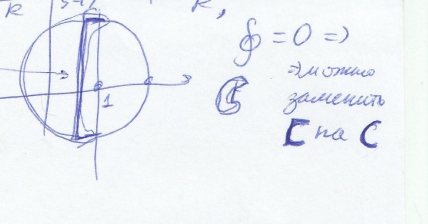
\includegraphics{p1.png}\q\\
\item $J(u) =  \frac{1}{2\pi i R} \IL_{[} f_u(s) u^{s-1} \os \frac{s-1}{R} + \frac{R}{s-1}  \cs ds $\\
$\lim\limits_{u\to\infty} J(u) = 0$\\
$g(s) = \frac{1}{2\pi i R}f(s)\os \frac{s-1}{R} + \frac{R}{s-1}    \cs $ ограничено на контуре, значит $\IL_{\TE+iR}^{1+iR}g(s) u^{s-1}ds \le \frac{\varepsilon}{\delta} $\\
Значит $|\IL_{BC} g(s)u^{s-1}ds |\le M2Ru^{\TE-1}\to0, u\to\infty\Ra \lim\limits_{u\to\infty}f_u(1) = f(1)\Ra $ интеграл сходится $\Ra$ асимптотический закон. $\pe$
\end{enumerate}
\end{mybox}



\newpage
\begin{mybox2}{\hypertarget{bil8}{Билет 8}}

\begin{formbox}{}
Доказательство асимптотического распределения распределения простых чисел. Асимптотическая формула $n$-го простого числа.
\end{formbox}
\begin{enumerate}
\item

\begin{formbox}{}
\begin{utv} $f(s) = -\frac{\zeta'(s)}{\zeta(s)} - \frac{1}{s-1} $ аналитическая при $\sigma \ge 1$
\end{utv}
\end{formbox}
$\pb$ Интересует $\sigma = 1$, т.к. при $\sigma > 1$ все ок.\\
$\exists$ окрестность, в которой функция аналитична.\\
$\zeta(s) = \frac{1}{s-1} + g(s),\q g(s)$  аналитичная.\\
$-\frac{-\zeta(s)}{s\zeta(s)} = -\frac{-\frac{1}{(s-1)^2} + g'(s)}{s\os \frac{1}{s-1} + g(s) \cs} = \frac{1}{s-1} \cdot \frac{1 - \overbrace{(s-1)^2}^{\to 0} g'(s)}{s (1 + (s-1)g(1))} = \frac{1}{s-1} + f(s)$, в $s = 1$ полюс первого порядка.$\pe$
\item Из преобразования Абеля $\sigma > 1$: $-\frac{\zeta'(s)}{\zeta(s)} - \frac{1}{s-1} = \IL_1^\infty\frac{\SI(x) - x}{x^{s+1}}dx\Ra f(s) = \IL_1^\infty\frac{\SI(x) - x}{x^{s+1}}dx $\\\q\\
\item $f_u(s) = \IL_1^u frac{\SI(x) - x}{x^{s+1}}dx$ -- целая, $u > 1$\\
$\pb \IL_a^b \frac{dx}{x^{s+k}} = \left.\frac{x^{-s-k+1}}{-s-k+1} \right|_a^b = \frac{b^{-s-k+1} - a^{-s-k+1}}{-s-k+1} = \frac{1 + (-s-k+1)\ln(b) + (-s-k+1)^2g(s) -1 - (-s-k+1)\ln(a)}{-s-k+1} $ -- нет особенностей, значит целая. ($\pm 1 $ сокращаются, а дальше числитель делится на знаменатель ура).$\pe$
\item Считаем вычет \\$\frac{1}{2\pi i R}\cdot \oint\limits_{\Gamma(\TE,R)}(f(s) - f_u(s)) u^{s-1}\os \frac{s-1}{R} + \frac{R}{s-1}  \cs ds = \frac{1}{R}\cdot (f(1) - f_u(1)) \cdot 1 \cdot R $
\item $\left| \frac{1}{2\pi i R} \IL_{C_R}F_k(s)ds \right| \le \frac{B}{R};\q\SI(x) \le Cx, |\SI(x) - x|\le (C+1)x = Bx$\\
$\pb |f(s) - f_u(s)| = \left| \IL_u^\infty \frac{\SI(x) - x}{x^{s+1}}dx   \right| \le \IL_u^\infty \frac{Bx}{x^{s+1}}dx = \left.B\frac{x^{1-\sigma}}{1-\sigma}\right|_u^\infty = \frac{Bu^{1-\sigma}}{\sigma - 1}  $\\
$\Ra \left| \frac{s-1}{R} + \frac{R}{s-1}  \right| = 2 |Re\frac{s-1}{R}| = 2 \frac{\sigma - 1}{R} \pe$
\item $\left| \frac{1}{2\pi i R}\IL_[ f_u(s)u^{s-1} \os   \frac{s-1}{R} + \frac{R}{s-1} \cs   \right| \le \frac{B}{R}$\\
При этом можно заменить [ на (, т.к. интеграл по ([ равен 0.\\
$|f_u(s)| = |\IL_1^u \frac{\SI(x)-x}{x^{s+1}}dx|\le B \frac{u^{1-\sigma}}{1-\sigma}$\\
$|  \frac{s-1}{R} + \frac{R}{s-1} | = 2 |Re \frac{s-1}{R}| = 2 \frac{1 - \sigma}{R}$
\end{enumerate}

\end{mybox2}
\newpage
\begin{mybox2}{{Билет 8}}
7. Рассмотрим $J(u) = \frac{1}{2\pi i R} \IL_[ f(s)u^{s-1} \os   \frac{s-1}{R} + \frac{R}{s-1} \cs ds$\\
Утверждается что предел равен 0.\\
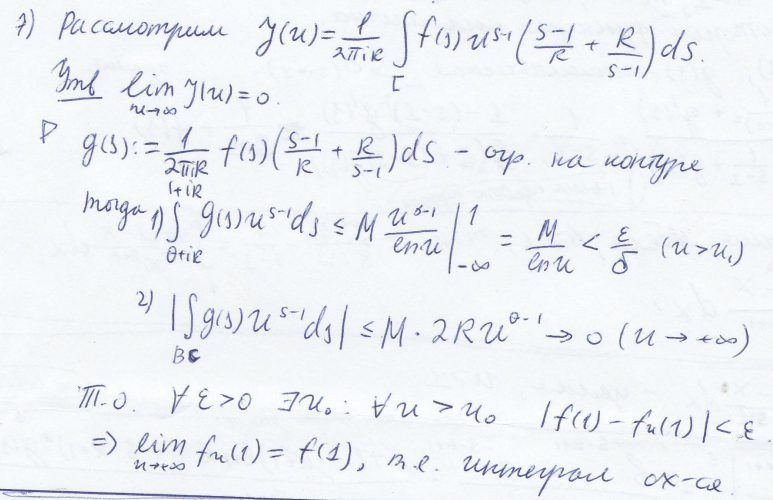
\includegraphics{p2.png}\q\\
/*я ничего не понял и мне лень писать сори:(*/
% \end{enumerate}

\begin{formbox}{}
\begin{utv} $p_n \sim n\ln(n)$ -- закон распределения $n$-того простого.
\end{utv}
\end{formbox}
$\pb n = \pi(p_n) = \frac{p_n}{\ln(p_n)}(1+\alpha_n) $\\
$\ln(n)  = \ln(p_n) - \ln(\ln(p_n)) + \ln(1+\alpha_n) = \ln(p_n)(1 + \beta_n)  $\\
$\Ra n\ln(n) = p_n(1 + \alpha_n)(1 + \beta_n) \pe $
\end{mybox2}



\newpage
\begin{mybox}{\hypertarget{bil9}{Билет 9}}

\begin{formbox}{}
Простейшие свойства сравнений. Группа $\os Z/mZ \cs ^*$. Теорема Эйлера. Малая теорема Ферма. Элементарные доказательства бесконечности множества простых чисел в прогрессиях вида $4n+1$ и $4n+3$.
\end{formbox}
\begin{formbox}{}
\begin{deff}[Сравнения]\q\\
$a \ee b \pmod{m}\iff m\mid (a-b) \iff a$ и $b$ дают одинаковые остатки при делении на $m$
\end{deff}
\end{formbox}
Свойства:
\begin{enumerate}
\item[0.] $a \ee b \pmod{m}\iff b \ee a \pmod{m}$
\item $a \ee b \pmod{m}\iff a + c \ee b + c\pmod{m}$
\item $a \ee b \pmod{m}\Ra ac \ee bc \pmod{m}$ !!!ТОЛЬКО В ОДНУ СТОРОНУ!!!
\item $\begin{cases} a \ee b \pmod{m}\\ c\ee d\pmod{m}\end{cases} \Ra a+c\ee b + d\pmod{m}$
\item $\begin{cases} a \ee b \pmod{m}\\ c\ee d\pmod{m}\end{cases} \Ra ac\ee bd\pmod{m}$
\item $ac\ee bc\pmod{mc}\Ra a\ee b\pmod{m}$
\item $ac\ee bc\pmod{m}, (m,c) = 1\Ra a\ee b\pmod{m}$
\end{enumerate}
Уравнение в факторкольце.\\
$\bb{Z}/m\bb{Z} = \{\bar{a}: \bar{a} = a + mt, t\in\bb{Z}\} \q\q a\ee b \iff \bar{a} = \bar{b}$\\
$\os \bb{Z}/m\bb{Z}  \cs^* = \{\bar{a}: \bar{a} = a + mt, (a,m) = 1\}$ !!ЭТО НЕ КОЛЬЦО, (т.к. нет сложения)!!! Но это группа по умножению: $1) \exists 1,\q 2) \exists a^{-1}$

\begin{formbox}{}
\begin{lem} $ax\ee b\pmod{m}, (a,m) = 1\Ra \exists!c<m:x\ee c\pmod{m}$
\end{lem}
\end{formbox}
$\pb 1) ax\ee b\pmod{m} $\\
$\exists u,v: au+mv = 1\Ra au \ee 1 \pmod{m} $\\
$a(bu) \ee b\pmod{m}$\\
$x\ee c\ee bu\pmod{m}$\\
$2)$ пусть их два разных:$x_1\not= x_2$\\
$ax_1\ee b\pmod{m}, ax_2\ee b\pmod{m}\Ra ax_1 \ee ax_2\pmod{m}\Ra x_1\ee x_2\pmod{m}\pe$

\begin{formbox}{}
\begin{teo}[Теорема Эйлера] $(a,m) = 1\Ra a^{\FI(m)} \ee 1\pmod{m}$
\end{teo}
\end{formbox}
\end{mybox}
\newpage
\begin{mybox}{{Билет 9}}
\begin{formbox}{}
\begin{teo}[Малая теорема Ферма] $p$-простое, $(p,a) = 1\Ra a^{p-1} \ee 1\pmod{p}$
\end{teo}
\end{formbox}
\begin{formbox}{}
\begin{utv} $p\mid (a^2+b^2), p\nmid a, p\not=2 \Ra p = 4m+1$
\end{utv}
\end{formbox}
$\pb a^2 + b^2 \ee 0\pmod{p}$\\
$a^2 \ee -b^2\pmod{p}, (a^2)^{\frac{p-1}{2}} \ee (b^2)^{\frac{p-1}{2}}\pmod{p}$\\
$a^{p-1}\ee b^{p-1} (-1)^{\frac{p-1}{2}} \Ra 1 \ee (-1)^{\frac{p-1}{2}}\pmod{p}\Ra \frac{p-1}{2} = 2m\Ra p = 4m+1\pe$

\begin{formbox}{}
\begin{utv} Бесконечность множества простых вида $4n-1$.
\end{utv}
\end{formbox}
$\pb $ Пусть их конечное число. Пусть $p_n$ -- максимальное из них.\\
Рассмотрим $p = 4(p_1\cdots p_n) - 1$ не простое. $\exists q\mid p:q = 4k-1$, т.к. если все делители имеют вид $4k+1$, то и $p \ee 1 \pmod{4}$, но $q \not= p_j$ противоречие.$\pe$

\begin{formbox}{}
\begin{utv} Бесконечность множества простых вида $4n+1$.
\end{utv}
\end{formbox}
$\pb $ Пусть $p_1,\dots,p_n$ -- все простые числа такого вида.\\
$(2p_1\cdots p_n)^2 + 1^2 = q_1\cdots q_m \Ra q_i = 4m_i+1$ по лемме, значит $q_i = p_j$ -- противоречие.$\pe$ 
\end{mybox}


\newpage
\begin{mybox2}{\hypertarget{bil10}{Билет 10}}

\begin{formbox}{}
Простейшие свойства групповых характеров. Построение характеров. Вычисление сумм $\sum_{a\in G} \chi(a)$ и $\sum_\chi \chi(a)$ для характеров $\chi$ группы $G$. Определение и свойства числовых характеров.
\end{formbox}
\begin{formbox}{}
\begin{deff} [Определение характера]\q\\
Пусть $G$ -- конечная группа, коммутативная по умножению.\\
$\chi:G\to\bb{C}$ -- характер
\begin{enumerate}
\item $\chi(g) \not\ee0 $
\item $\chi(g_1 \cdot g_2) = \chi(g_1)\cdot \chi(g_2)  $
\end{enumerate}
\end{deff}
\end{formbox}
Свойства характеров.
\begin{enumerate}
\item $\chi(e) = 1\q\q \pb \chi(e\cdot e) = \chi(e)\cdot \chi(e) \pe$
\item $g^h=e\Ra (\chi(g))^h = 1 \Ra $ характеры принимают значения только корней из 1.
\item $\chi(g^{-1}) = \frac{1}{\chi(g)}$
\end{enumerate}
 $\chi_0(g)\ee 1$ -- главный характер.\\
 $\chi_1 \chi_2 (g):= \chi_1(g)\cdot\chi_2(g)$\\

Характеры образуют группу относительно операции \(\chi_1 \chi_2 (g)\)
$\pb$
\begin{enumerate}
\item $\chi_1\chi_2 (g_1 g_2) = \chi_1(g_1)\chi_1(g_2)\chi_2(g_1)\chi_2(g_2) = \chi_1\chi_2(g_1)\chi_1\chi_2(g_2)$
\item $\exists \chi^{-1}: \chi^{-1}(g) =\chi(g^{-1}) = \frac{1}{\chi(g)}$
\item $\exists 1: \chi\chi^{-1}(g) = 1$
\item $(\chi_1\chi_2)\chi_3 (g) = \chi_1(\chi_2\chi_3) (g)$\\$\pb (\chi_1\chi_2)\chi_3 (g) = (\chi_1(g)\chi_2(g))\chi_3(g) = \chi_1(g)(\chi_2(g)\chi_3(g)) = \chi_1(\chi_2\chi_3) (g)\pe$
\end{enumerate} $\pe$\\
Пусть $G = G_1\otimes \cdots \otimes G_n$, где все $G_i$ циклические. $ord g_i = h_i$\\
$ord (G) = h = h_1\cdots h_n$\\
$\forall g\in G: g = g_1^{r_1}\cdots g_n^{r_n},\q\q 0\le r_i\le h_i$ и такое представление единственно.\\
\end{mybox2}
\newpage
\begin{mybox2}{{Билет 10}}
\begin{formbox}{}
Рассмотрим набор корней из 1:$\zeta_1,\dots,\zeta_n: \zeta_i^{h_i} = 1$\\
$\chi(g) = \zeta_1^{r_1}\cdots \zeta_n^{r_n}$


\begin{utv} Это характер и любой характер можно записать так.
\end{utv}
\end{formbox}
$\pb 1) g = g_1^{k_1}\cdots g_n^{k_n}\q\q k_j = r_j + a_jh_j\Ra g = g_1^{r_1}\cdots g_n^{r_n} $ а дальше рассмотрим характер и такие ого записался.\\
$2) a = g_1^{a_1}\cdots g_n^{a_n};\q b = g_1^{b_1}\cdots g_n^{b_n}$\\
$ab = g_1^{a_1 + b_1}\cdots g_n^{a_n + b_n}$ и получаем что характер произведения равен произведению характеров. Проверили. $\pe$

Если $\chi \not=\chi_0$, то $\exists g: \chi(g) \not=1$\\
Если $g\not=e$, то $\exists \chi: \chi(g)\not=1$

\begin{formbox}{}
\begin{utv}\q\\
\begin{enumerate}
\item $S = \SL_{g\in G}\chi(g) = \begin{cases}h, \chi = \chi_0\\ 0, \chi \not= \chi_0\end{cases}$
\item $\sigma = \SL_{\chi}\chi(g) = \begin{cases}h, g = e\\ 0, e \not= e\end{cases}$
\end{enumerate}
\end{utv}
\end{formbox}
$\pb$ Сначала рассмотрим тривиальные случаи:\\
$\chi = \chi_0\Ra\chi(g) = 1\Ra S = |G| = h$\\
$g = e\Ra \chi(e) = 1\Ra\sigma = |G| = h$\\
Теперь остальные:\\
$\chi \not=\chi_0 \Ra \exists a\in G: \chi(a)\not=1$\\
$\chi(a)S = \SL_{g\in G}\chi(a)\chi(g) = S\Ra (\chi(a) - 1) S = 0 \Ra S = 0$\\\q\\
$g\not=e\Ra\exists \chi_1:\chi_1(g)\not=1$\\
$\chi_1(g)\sigma = \sigma \Ra \sigma = 0 \pe$

Числовые характеры.\\
$\bb{Z}_m^* = \os \bb{Z}/m\bb{Z}  \cs^* = \{\bar{a}: \bar{a} = a + mt,\q (a,m) = 1 \}, \bar{a}\bar{b} = \overline{ab}  $\\
$\chi(x) = \begin{cases} \chi(\bar{x}), (x,m)=1\\0,(x,m) \not=1 \end{cases} $\\
$\chi_0(x) = \begin{cases} 1, (x,m)=1\\0,(x,m) \not=1 \end{cases} $\\\q\\
$a\ee b \pmod{m} \Ra \chi(a) = \chi(b) $\\
\end{mybox2}
\newpage
\begin{mybox2}{{Билет 10}}
$\chi(ab) = \chi(a)\chi(b) $\\
$\chi(a)\not=0 \iff (a,m)=1$\\\q\\
$\SL_{x=1}^m \chi(x) = \begin{cases} \FI(m), \chi = \chi_0\\0 \end{cases} $\\
$\SL_{\chi} \chi(x) = \begin{cases} \FI(m), x = 1\\0 \end{cases} $\\
$\left|\SL_{x=1}^{r} \chi(x) \right| = \left|\SL_{x=mq+1}^{mq+r} \chi(x)\right|\le r\le m$
\end{mybox2}





\newpage
\begin{mybox}{\hypertarget{bil11}{Билет 11}}

\begin{formbox}{}
Аналитичность функции Дирихле $L(s,\chi)$ в области $\sigma > 1$. Разложение в ряд Дирихле ее логарифмической производной. Отсутствие нулей $L$-функции в области $\sigma > 1$. Представление $L$-функции в виде бесконечного произведения. Аналитическое продолжение функции $L(s,\chi_0)$ в область $\sigma > 0$.
\end{formbox}
\begin{formbox}{}
\begin{deff}
$L(s,\chi) = \SL_{n=1}^\infty \frac{\chi(n)}{n^s}$ -- функция Дирихле.
\end{deff}
\end{formbox}
$\zeta(s) = \SL_{n=1}^\infty \frac{1}{n^s};$ если $\SL_{n=1}^\infty f(n) = A, \SL_{d=1}^\infty f(d)\Lambda(d) = B$ -- абсолютно сходящийся ряд. $\Lambda(n) = \begin{cases} \ln(p), n=p^k\\0  \end{cases} \q\q \Ra AB = \SL_{n=1}^\infty f(n)\ln(n)$\\\q\\
$\SL_{n=1}^\infty f(n) = \prod\limits_p \os 1 - f(p)\cs^{-1}$.\\ Если $f(n) = \frac{\chi(n)}{n^s}\Ra L(s,\chi) = \prod\limits_p \os 1 - \frac{\chi(p)}{p^s}   \cs^{-1} $\\
$L(s,\chi) \cdot \SL_{n=1}^\infty \frac{\chi(n)\Lambda(n)}{n^s} = \SL_{n=1}^\infty \frac{\chi(n)\ln(n)}{n^s}  = -L'(s,\chi)\Ra $ в области $\sigma > 1: L(s,\chi)\not=0$\\
$\chi_0(p) = \begin{cases} 1, (m,p) = 1\\0  \end{cases}\Ra L(s,\chi) = \prod\limits_{p\nmid m}(1 - \frac{1}{p^s})^{-1} $\\
$L(s,\chi_0) = \zeta(s) \prod\limits_{p\mid m} (1 - \frac{1}{p^s})^{-1} = \os \frac{1}{s-1} + f(s) \cs  \prod\limits_{p\mid m} (1 - \frac{1}{p^s})^{-1} = \frac{a_m}{s-1} + f_m(s),\\ a_m = \prod\limits_{p\mid m} (1 - \frac{1}{p^s}) = \frac{\FI(m)}{m} > 0 \Ra  L(s,\chi_0)$  аналитична в области $\sigma > 0$
\end{mybox}


\newpage
\begin{mybox2}{\hypertarget{bil12}{Билет 12}}

\begin{formbox}{}
Теорема о почленном дифференцировании ряда Дирихле. Область аналитичности функции $L(s, \chi)$ при $\chi \not= \chi_0$.
\end{formbox}
Рассмотрим область $D(\delta, \TE) = \begin{cases} \sigma > \delta > 0\\|arg(s)| < \TE, \TE \in (0, \frac{\pi}{2})\end{cases}$\\
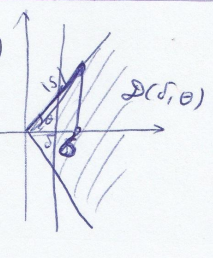
\includegraphics{p3.png}\q\\

\begin{formbox}{}
\begin{utv}\q\\
\begin{enumerate}
\item Ряд $\SL_n \frac{a_n}{n^s} $ равномерно сходится в $D(\delta, \TE)$
\item $f(s)$ аналитична в области $\sigma > 0,$ где $f(s) = \SL_n\frac{a_n}{n^s}$
\end{enumerate}
\end{utv}
\end{formbox}
$\pb$ Определение равномерной сходимости: $\forall \varepsilon > 0 \exists M(\varepsilon): \forall N > M, \forall s\in D(\delta, \TE): \left|R_N(s)\right| = \left|\SL_{n = N+1}^\infty \frac{a_n}{n^s}\right| < \varepsilon$\\
Перепишем: $R_N(s) = \SL_{k=0}^\infty \frac{a_{N+k}}{(N+k)^s}\q\q A(x) = \SL_{k\le x}a_k; g(x) = \frac{1}{(N+x)^s}$\\
$|A(x)| \le 2C; \q g(x) \to 0\Ra A(x)g(x)\to0$\\
$g'(x) = -s(N+x)^{-s-1}, s\IL_1^\infty A(t)(N+t)^{-s-1}dt $ сходится, значит можно использовать преобразование Абеля.\\
$\SL_{k=1}^\infty g(k) a_k = -\IL_1^\infty A(t) g'(t) dt = -s\IL_1^\infty A(t)(N+t)^{-s-1}dt = R_N(s) $\\
$\left|R_N(s)\right| \le |s|\IL_1^\infty 2C(N+t)^{-s-1}dt = |s| \cdot 2C\left.\frac{(N+t)^{-\sigma}}{-\sigma}\right|_1^\infty = 2C\frac{(N+1)^{-\sigma}}{\sigma}|s|$\\
В области $D(\delta, \TE): \q \left|R_N(s)\right|\le 2CN^{-\delta}\frac{1}{\cos(\TE)} < \varepsilon \Ra$ выполняется равномерная сходимость.\\
Для любой точки правее нуля можно подобрать такие $\delta$ и $\TE$, чтобы она попала в область. Раз в таких областях ряд сходится равномерно, значит его можно дифференцировать бесконечное число раз, значит функция аналитична.$\pe$

\end{mybox2}





\newpage
\begin{mybox}{\hypertarget{bil13}{Билет 13}}

\begin{formbox}{}
Теорема об области сходимости ряда Дирихле с неотрицательными коэффициентами.
\end{formbox}
Пусть есть  ряд $f(s) = \sum a_n n^{-1}, \q \sigma_1 < \sigma_2 < \sigma_0$\\

\begin{formbox}{}
\begin{teo} Пусть функция $f(s) = \SL_{n=1}^\infty \frac{a_n}{n^s}, \sigma_1 <\sigma_2 < \sigma_0 $
\begin{enumerate}
\item $f(s)$ аналитична при $\sigma > \sigma_1$
\item $f(s) = \SL_{n=1}^\infty  \frac{a_n}{n^s},\q(\sigma > \sigma_2) $
\item $a_n \ge 0$
\end{enumerate}
Тогда $f(s)$ раскладывается в ряд Дирихле при $\sigma > \sigma_1$ и его можно почленно дифференцировать. $///<WTF?$\\
/*P.S. в другом источнике: Тогда $f(s)$ аналитична при $\sigma > \sigma_1$, т.е. можно продлить представление рядом.*/
\end{teo}
\end{formbox}
$\pb $ Если $f(s) \sum \frac{a_n}{n^s}$ сходится при $s = s_0 = \sigma_0 + it_0$, то ряд Дирихле задаёт функцию, аналитичную в области $\sigma > \sigma_0\Ra$ можно дифференцировать.\\
$\Ra$ есть прямая, разделяющая области сходимости и расходимости.\\
Рассмотрим $\sigma_0 > \sigma_2$,  разложим в ряд Тейлора:\\
$f(s) = \SL_{k=0}^\infty \frac{f^{(k)}(\sigma_0)}{k!} (s - \sigma_0)^k $\\
Берем $\sigma\in(\sigma_1, \sigma_2)$ и подставляем вместо $s$. (анализируем сходимость в $\sigma > \sigma_1$)\\
$f(\sigma) = \SL_{k=0}^\infty \frac{f^{(k)}}{k!}(\sigma - \sigma_0)^k = \SL_{k=0}^\infty \SL_{n=1}^\infty \frac{a_n (-\ln(n))^k}{n^{\sigma_0}} \frac{1}{k!} (\sigma - \sigma_0)^k   = \SL_{k=0}^\infty \frac{(\sigma - \sigma_0)^k}{k!}\SL_{n=1}^\infty \frac{a_n (-\ln(n))^k}{n^{\sigma_0}} = \SL_{n=1}^\infty \frac{a_n}{n^{\sigma_0}} \SL_{k=0}^\infty \frac{\os(\sigma_0 - \sigma)\ln(n)\cs^k}{k!}  = \SL_{n=1}^\infty \frac{a_n}{n^{\sigma_0}} e^{(\sigma - \sigma_0)\ln(n)} = \SL_{n=1}^\infty \frac{a_n}{n^\sigma} $\\
Ряд задает аналитическую функцию по теореме единственности аналитического продолжения функции заданной этим рядом при $\sigma > \sigma_1 \pe$
\end{mybox}



\newpage
\begin{mybox2}{\hypertarget{bil14}{Билет 14}}

\begin{formbox}{}
Неравенство $L(1,\chi)\not=0$ для действительного характера $\chi$.
\end{formbox}
\begin{formbox}{}
\begin{deff} Характер $\chi$ действительный, если $\chi^2 = \chi_0 = 1$
\end{deff}
\end{formbox}
\begin{formbox}{}
\begin{lem} $f(s):= \zeta(s) L(s,\chi) \Ra$
\begin{enumerate}
\item $f(s) = \SL_{n=1}^\infty \frac{a_n}{n^s},\q\sigma > 1 $
\item $a_n \ge 0$
\item $a_{n^2} \ge 1$
\item $\SL_{n=1}^\infty \frac{a_n}{\sqrt{n}} $ расходится.
\end{enumerate}
\end{lem}
\end{formbox}
$\pb f(s) = \SL_{k=1}^\infty \frac{1}{k^s}  \SL_{d=1}^\infty \frac{\chi(d)}{d} = \SL_{n=1}^\infty \frac{1}{n^s} \SL_{d\mid n}\chi(d)$\\
Если $n = p_1^{k_1}\cdots p_r^{k_k}$, то $a_n = \SL_{d\mid n}\chi_d  \prod\limits_{j=1}^n (1 + \chi(p_j) + \chi(p_j^2) + \cdots)  = \prod\limits_{j=1}^n (1 + \chi(p_j) + \chi(p_j^2) + \cdots) =  \prod\limits_{j=1}^n (1 + \chi(p_j) + \chi^2(p_j) + \cdots)$\\
где $a_{n_j} = \begin{cases} 1, &\chi(p_j) = 0\\k_j + 1, &\chi(p_j)=1\\1, &\chi(p_j) = -1, k_j=2m\\0 &\chi(p_j) = -1, k_j=2m+1 \end{cases}$\\
Если $n = k^2,$ то все $k_j=2m\Ra$\\
$\prod\limits_{j=1}^r  a_{n_j} \ge 1 \Ra 1)+2)+3)$ ////<WTF??\\
$4) \SL_{n=1}^\infty \frac{a_n}{\sqrt{n}} \ge \SL_{k=1}^\infty \frac{a_{k^2}}{k}  \Ra$ расходится. $\pe$

\begin{formbox}{}
\begin{teo} $\chi$-- действительный характер, тогда $L(1, \chi) \not=0$
\end{teo}
\end{formbox}
$\pb L(1,\chi) = 0\Ra L(s\chi) = (s-1)g(s), \q g(s)$ аналитичная\\
$\zeta(s) =\frac{1}{s-1} + h(s) $ -- тоже аналитичная\\
$f(s) = \zeta(s) L(s,\chi) = g(s) + g(s)h(s)(s-1)  $ представляется сходящимся рядом Дирихле в $\sigma > 0$ а это противоречие с пунктом 4 леммы $\pe$ 
\end{mybox2}





\newpage
\begin{mybox}{\hypertarget{bil15}{Билет 15}}

\begin{formbox}{}
Неравенство $L(1,\chi)\not=0$ при $\chi^2\not=\chi_0$.
\end{formbox}
\begin{formbox}{}
\begin{lem} Пусть $s\in \bb{R}, s > 1$, тогда $A:= |L^3(s,\chi_0)\cdot L^4(s,\chi)\cdot L(s, \chi^2)| \ge 1$
\end{lem}
\end{formbox}
$\pb L(s, \chi) = \prod\limits_p \os 1 - \frac{\chi(p)}{p^s} \cs ^{-1} $\\
$A = \prod\limits_{p\mid m} \left|\os 1 - \frac{1}{p^s} \cs^3  \os 1 - \frac{\chi(p)}{p^s} \cs^4  \os 1 - \frac{\chi^2(p)}{p^s} \cs^3  \right|^{-1}   $\\
Из \hyperlink{bil6}{билета 6} $|(1-r)^3 (1-re^{i\varphi})^4 (1 - re^{2i\FI})| \le 1 \q\q\Ra r = \frac{1}{p}\Ra \pe$

\begin{formbox}{}
\begin{teo} При $\chi \not= \chi_0: L(1,\chi)\not=0$
\end{teo}
\end{formbox}
$\pb L(1,\chi) = 0\Ra L'(1,\chi) = \lim\limits_{s\to1+0} \frac{L(s,\chi) - L(1,\chi)}{s-1} = \lim\limits_{s\to1+}\frac{L(s,\chi)}{s-1}\Ra \left| \frac{L(s,\chi)}{s-1} \right| \le C_1$\\
$L(s, \chi_0) = \SL_{(m,n) = 1}^\infty \frac{1}{n^s} < \zeta(s) \le \frac{2}{s-1} $\\
$L(s,\chi) = (s-1)g_m(s) $\\
$|L(s,\chi)| \le C_1(s-1)\q\q |L(s,\chi^2)| \le C_2$\\
$1 \le A\le \left| \os  \frac{2}{s-1} \cs^3 (C_1 (s-1))^4 C_2  \right| \to 0$ противоречие. $\pe$

\end{mybox}



\newpage
\begin{mybox2}{\hypertarget{bil16}{Билет 16}}

\begin{formbox}{}
Доказательство теоремы Дирихле о бесконечности множества простых чисел в арифметической прогрессии.
\end{formbox}
\begin{formbox}{}
\begin{teo}[Теорема Дирихле] Пусть $m\ge 2$. В прогрессии $mx+l, (m,l) = 1$ бесконечно много простых.
\end{teo}
\end{formbox}
$\pb F(s) = \SL_{\chi}\chi(u) \os -\frac{L'(s,\chi)}{L(s,\chi)}  \cs, \q\q s\in\bb{R}, s > 1 $\\
$u$ выбрали так, что $lu\ee 1\pmod{m}$\\
\begin{enumerate}
\item На $(1,2)\q F(s)$ не ограничена\\
$F(s) = -1 \frac{L'(s,\chi_0)}{L(s,\chi)} + \SL_{\chi\not=\chi_0} \chi(u) \frac{L'(s,\chi_0)}{L(s,\chi)}  = \frac{1}{s-1} + G(s),\q\q G(s) $ ограничена при $\sigma > 1$
\item Если количество простых конечно, то $F(s)$ ограничена на $(1,2)$\\
$-\frac{L'(s,\chi)}{L(s,\chi)} = \SL_{n=1}^\infty \frac{\Lambda(n)\chi(n)}{n^s}\Ra F(s) = \SL_{\chi} \chi(u) \SL_{n=1}^\infty \frac{\Lambda(n)\chi(n)}{n^s} = \SL_{n=1}^\infty \frac{\Lambda(n)}{n^s} \SL_\chi \chi(un) = \FI(m) \SL_{un\ee1\pmod{m}} \frac{\Lambda(n)}{n^s}  =  \FI(m) \SL_{n\ee l\pmod{m}} \frac{\Lambda(n)}{n^s} = \FI(m)\SL_{p\ee l\pmod{m}} \frac{\ln(p)}{p^s} + R(s)$\\
$0 \le R(s)  = \FI(m)\SL_{p}\SL_{k=2, p^k \ee l\pmod{m}}  \frac{\ln(p)}{p^s}\le \FI(m)  \SL_{p=2}^\infty \frac{\ln(p)}{p(p-1)} \le C $\\
То есть $F(s) = \FI(m) \SL_{p\ee l\pmod{m}} \frac{\ln(p)}{p(p-1)} + O(1) $\\
Если число простых конечно, то $F(s) $ ограничена. Противоречие.$\pe$
\end{enumerate}

\end{mybox2}



\newpage
\begin{mybox}{\hypertarget{bil17}{Билет 17}}

\begin{formbox}{}
Свойства минимального многочлена алгебраического числа. Целые алгебраические числа. Лемма Гаусса и ее следствия, относящиеся к целым алгебраическим числам.
\end{formbox}
\begin{formbox}{}
\begin{lem} Если $\FI(x)\in\bb{Q}[x]   $ имеет общий корень с неприводимым многочленом $f(x)$, то $f(x)$ -- делитель $\FI(x)\Ra $ каждый корень $f(x)$ является корнем $\FI(x)$
\end{lem}
\end{formbox}
$\pb m = deg(\FI), \q n = deg(f)$\\
Если $m = 0,$ то $\FI\ee 0$. Пусть теперь $m > 0$\\
Тогда $\FI(x) = q(x)f(x) + r(x), deg(r) < n$\\
$x = \AL$ -- общий корень, тогда $0 = \FI(\AL) = q(\AL)f(\AL) + r(\AL) \Ra r \ee 0 \Ra \FI(x) = q(x)f(x)  \pe$ 

\begin{formbox}{}
\begin{lem} Неприводимый многочлен $f(x)\in\bb{Q}[x]$ не может иметь кратных корней.
\end{lem}
\end{formbox}
$\pb f(x)$ имеет кратные корни, тогда $f(x)$ имеет общий корень с $f'(x)$, значит делится на $f'$, значит он не был неприводимым.$\pe$ 

\begin{formbox}{}
\begin{deff} Число $\AL$ -- алгебраическое, если оно является корнем многочлена с рациональными коэффициентами, иначе трансцендентное.\\
Степень алгебраического числа $\AL$ -- степень неприводимого многочлена, имеющего корень $\AL$
\end{deff}
\end{formbox}

$\forall n \q\exists$ неприводимый многочлен степени $n$ (например $x^n - 2$), значит существуют алгебраические числа любой степени.

\begin{formbox}{}
\begin{deff} Пусть $\AL$ -- алгебраическое число степени $n, \exists f\in\bb{Q}[x], deg(f) = n, \AL$ -- корень $f$, старший коэффициент $f = 1$, тогда $f$ -- минимальный многочлен.\\
Корни $\AL_1,\dots,\AL_n$ минимального многочлена -- сопряженные с $\AL$ 
\end{deff}
\end{formbox}
Свойства сопряженных чисел.\\
\begin{enumerate}
\item $\AL_1,\dots,\AL_n$ -- алгебраические числа одинаковой степени с одинаковым минимальным многочленом
\item $\AL_1,\dots,\AL_n$  сопряженные все друг другу.
\item $\AL_1,\dots,\AL_n$ различны.
\end{enumerate}

\end{mybox}
\newpage
\begin{mybox}{{Билет 17}}
\begin{formbox}{}
\begin{utv} $B(x) \in \bb{Q}[x], A(x) $ -- минимальный многочлен $\AL$, $\forall$ корня $B(x)$ это корень $A(x)\Ra B(x) = \Lambda  A^m(x)$
\end{utv}
\end{formbox}
$\pb B(x) = A(x)B_1(x), \forall x: B_1(x) = 0: A(x) = 0 \Ra B(x) = A^2(x)B_2 \cdots \pe$


\begin{formbox}{}
\begin{deff} Если $A(x)\in\bb{Z}[x]$, старший коэффициент = 1 -- минимальный многочлен для $\AL$, то $\AL$ -- целое алгебраическое число.
\end{deff}
\end{formbox}
\begin{formbox}{}
\begin{teo} Пусть $B(x) \in \bb{Z}[x], b_n = 1, B(\AL) = 0 \Ra \AL$ -- целое алгебраическое.
\end{teo}
\end{formbox}
\begin{formbox}{}
\begin{deff} $A(x) = a_nx^n + \cdots + a_0\in\bb{Z}$ примитивный, если $(a_0,\dots,a_n) = 1$
\end{deff}
\end{formbox}
\begin{formbox}{}
\begin{lem}[Гаусса] $A(x),B(x)$ примитивные, тогда $C(x) = A(x)B(x)$ тоже примитивный.
\end{lem}
\end{formbox}
$\pb B(x) = b_mx^m + \cdots b_0,\q\q A(x) = a_nx^n+\cdots +a_0$\\
Покажем, что $\forall p: \exists c_j: p\nmid c_j$\\
$\forall p \exists a_s, b_t: p\nmid a_s, p\nmid b_t, p\mid a_0, \dots a_n, b_0,\dots b_m$.\\
Тогда $c_{s+t} = \SL_{k+l = s+t} a_kb_l = \underbrace{a_sb_t}_{\not\divisible p} + \underbrace{\SL resid}_{\divisible p} \not\divisible p\pe$
Доказательство теоремы.\\
$B(x)$ обнуляется $\AL; A(x) = x^n + \cdots a_0 \in\bb{Q}[x]$ -- минимальный многочлен $\AL$. Тогда $B(x) = A(x)C(x) = \frac{u}{v} \tilde{A}(x)\tilde{C}(x) $, где с тильдами целые. Тогда $\tilde{A}, \tilde{C}$ -- примитивные, значит $vB(x)$ тоже примитивный. По лемме Гаусса $v = 1\Ra \tilde{A}\tilde{C} = B\Ra \tilde{A}$ -- минимальный целый многочлен, значит $\AL$ -- целое алгебраическое число.$\pe$

\end{mybox}








\newpage
\begin{mybox2}{\hypertarget{bil18}{Билет 18}}

\begin{formbox}{}
Формулировка основной теоремы о симметричных многочленах. Теорема о симметричном многочлене от нескольких систем сопряженных алгебраических чисел. Поле алгебраических чисел и кольцо целых алгебраических чисел. Алгебраическая замкнутость поля алгебраических чисел.
\end{formbox}
Пусть $K$ -- коммутативное кольцо с 1, $K[\AL_1, \dots, \AL_n]$ -- кольцо многочленов с коэффициентами из $K$ от $\AL_1,\dots,\AL_n$.\\


\begin{formbox}{}
\begin{deff} Многочлен $P(\AL_1,\dots,\AL_n) \in K[\AL_1, \AL_n]$ симметрический, если он не изменяется при любой перестановке переменных.
\end{deff}
\end{formbox}
Обозначим $\sigma_1 = \AL_1 +\cdots + \AL_n; \sigma_2 = \AL_1\AL_2 \cdots \AL_{n-1}\AL_n; \cdots; \sigma_n = \AL_1\cdots\AL_n$ -- элементарные симметричные многочлены. С точностью до знака это коэффициенты $(x-\AL_1)\cdots(x-\AL_n)$

\begin{formbox}{}
\begin{teo} [о симметричных многочленах] Любой симметричный многочлен от переменных $\AL_1, \dots, \AL_n$  единственным образом представляется в виде $P(\AL_1,\dots,\AL_n) = H(\sigma_1, \dots, \sigma_n),$ где $H\in K[\sigma_1, \dots, \sigma_n], \q \sigma_1, \dots, \sigma_n$ -- элементарные симметричные.
\end{teo}
\end{formbox}

Рассмотрим несколько систем переменных $\AL_1,\dots,\AL_n, \delta_1,\dots,\delta_s$; Пусть $\sigma_1, \dots, \sigma_n, \eta_1,\dots,\eta_s$ -- их элементарные симметричные многочлены.

\begin{formbox}{}
\begin{deff} $P(\AL_1, \dots, \AL_n, \delta_1,\dots,\delta_s)$ -- симметричный многочлен относительно нескольких систем переменных, если он не изменяется при любой перестановке внутри каждой системы.
\end{deff}
\end{formbox}
\begin{formbox}{}

\begin{teo} [о симметричных многочленах от нескольких систем] Любой симметричный многочлен от нескольких систем переменных $\AL_1, \dots, \AL_n, \delta_1,\dots,\delta_m$  единственным образом представляется в виде $P(\AL_1,\dots,\AL_n,\delta_1,\dots,\delta_m) = H(\sigma_1, \dots, \sigma_n, \eta_1,\dots, \eta_m),$ где $\sigma_1, \dots, \sigma_n, \eta_1,\dots, \eta_m$ -- элементарные симметричные.
\end{teo}
\end{formbox}
$\pb $ считаем все переменные кроме $\AL_1,\dots,\AL_n$ константами, тогда $P = H_1(\sigma_1, \dots, \sigma_n, \eta_1,\dots, \eta_m)$, далее рассмотрим коэффициенты и будем их рассматривать как симметричные с меньшим числом систем, значит доказали по индукции. (база индукции предыдущая теорема и я хз где доказательство...)$\pe$ 

\end{mybox2}
\newpage
\begin{mybox2}{{Билет 18}}
\begin{formbox}{}
\begin{lem} Пусть $\AL,\dots,\delta$ -- алгебраические числа, $\AL_1,\dots,\AL_n,\delta_1,\dots,\delta_m$ -- соответствующие сопряженные. $P(x,\AL_1,\dots, \delta_m)\in\bb{Q}[x,\AL_1,\dots, \delta_m]$ -- симметрический относительно систем. Тогда $P\in\bb{Q}[x]$, т.е. не зависит от корней, а если не зависит от х, то тоже  $\in\bb{Q}[x]$%Тогда он не зависит от $\AL, \delta$
\end{lem}
\end{formbox}
$\pb$ Рассмотрим $P$ как многочлен от $\AL_1,\dots,\delta_m$ с коэффициентами из $\bb{Q}$. Элементарные многочлены с точностью до знака -- коэффициенты минимального многочленов, т.е. числа из $\bb{Q}\Ra P\in\bb{Q}[x]\pe $///<WTF??

\begin{formbox}{}
\begin{teo}
Если $\AL, \beta$ -- алгебраические числа, то $\AL+\beta, \; \AL-\beta,\; \AL\beta, \; \frac{\AL}{\beta}\; (\beta \not=0)$ -- тоже алгебраические. (что значит что множество алгебраических чисел образуют поле)
\end{teo}
\end{formbox}
$\pb$ Рассмотрим $P_1(x) = \prod\limits_{i=1}^n\prod\limits_{j=1}^s (x - (\AL_i \pm \beta_j)) $. Это симметричный многочлен по системам переменных $\AL, \beta$\\
$P_2(x) = \prod\limits_{i=1}^n\prod\limits_{j=1}^s (x - \AL_i\beta_j)$\\
По лемме $P_1, P_2\in\bb{Q}[x]$\\
$\frac{\AL}{\beta} = \AL\cdot \beta^{-1}\pe$\\P.S. Кажется что $\beta^{-1}$ тоже алгебраическое, потому что мы в минимальном для $\beta$ заменим все коэффициенты в разложении на $\frac{1}{\beta_i}$.\\
Следствие: $deg(\AL\pm\beta), deg(\AL\beta), deg(\frac{\AL}{\beta}) \le deg(\AL) deg(\beta) $


\begin{formbox}{}
\begin{deff} $A$ -- поле алгебраических чисел, расширение поля $\bb{Q}$
\end{deff}
\end{formbox}
\begin{formbox}{}

\begin{teo} $A$ -- алгебраически замкнутое (и любой многочлен разлагается на линейные множители), т.е. если $\xi$ -- корень $\FI(x) = x^m + \AL x^{m-1} + \cdots + \delta, \q\AL,\dots,\delta $ -- алгебраические, то $\xi$ алгебраическое.
\end{teo}
\end{formbox}
$\pb$ Рассмотрим $P(x) =\prod\limits_{i=1}^n\cdots\prod\limits_{l=1}^s (x^m + \AL_i x^{m-1} + \cdots + \delta_l)$ -- симметричный от систем переменных с коэффициентами из $\bb{Z}$. По лемме $P(x)\in\bb{Q}[x]$. $P(x)\divisible \FI(x) \Ra P(\xi) = 0 \Ra \xi$ алгебраическое. $\pe$

\end{mybox2}








\newpage
\begin{mybox}{\hypertarget{bil19}{Билет 19}}

\begin{formbox}{}
Алгебраическое числовое поле конечной степени. Каноническая форма представления его элементов. Теорема о числах, сопряженных в алгебраическом числовом поле. Теорема о примитивном элементе.
\end{formbox}
Пусть $C(x)$ -- минимальный многочлен для $\TE$ степени $n$.\\
$Q(\TE) = \left\{  \frac{f(\TE)}{g(\TE)}, \q f(x), g(x) \in\bb{Q}[x], g(\TE)\not=0 \right\} $

\begin{formbox}{}
\begin{teo} $Q(\TE) = \{r_{n-1}(\TE), r_{n-1}(\TE)\in\bb{Q}[x], deg(r_{n-1})\le n - 1\q\} $
\end{teo}
\end{formbox}
$\pb \AL = \frac{f(\TE)}{g(\TE)}, \q (C(x), g(x)) = 1$, т.к. если есть общий корень, то $g(\TE) = 0$\\
$\exists u,v \in\bb{Q}[x]: ug+vC = 1$\\
$\underbrace{C(\TE)}_{=0}v(\TE) + g(\TE)u(\TE) = 1\Ra g(\TE) = \frac{1}{u(\TE)}  $\\
Тогда $\AL = f(\TE)u(\TE) = h(\TE);\q h = qC+r_{n-1}\Ra \AL:=r_{n-1} \pe$\\\q\\
Следствие: $Q(\TE) = <\{1, \TE, \TE^2, \dots, \TE^{n-1}\}>$ -- алгебраическое числовое поле конечной степени, $n$ -- степень поля.\\
Рассмотрим $r_{n-1}(\TE_j)$ (б.о.о. $\TE = \TE_1$). Обозначим $r_{n-1}: r$. Положим $r(\TE_1) = \AL,\q \AL_1,\dots, \AL_n$ -- сопряженные с $\AL$.\\

\begin{formbox}{}
\begin{teo} $r(\TE_1),\dots,r(\TE_n)$ -- тот же набор, что и $\AL_1, \dots, \AL_m, \frac{n}{m}\in\bb{N}$%\q ////<< WWTTFF??
\end{teo}
\end{formbox}
$\pb P(x) = (x - r(\TE_1))\cdots(x - r(\TE_n)) \in \bb{Q}[x] $\\
Пусть $A$ -- минимальный многочлен для $\AL$\\
$A(r(\TE)) = A(\AL) = 0 \Ra$ у $A(r(x))$ все сопряженные $\TE$ тоже корни.\\
Любой корень $P$ -- корень $A\Ra P(x) = \lambda A^k(x), \lambda = 1$\\
Тогда $deg(P) = n = km \Ra k = \frac{n}{m}\in\bb{N} \pe$\\
Следствие. $\AL\in K \Ra deg(\AL) \mid deg(\TE) = deg(K)$ (т.е. в расширении с $\sqrt[3]{2}$ квадратных корней нет).

\begin{formbox}{}
\begin{deff} $\AL = r(\TE)\Ra N(\AL) := r(\TE_1)\cdots r(\TE_n)$ -- норма алгебраических чисел в поле.
\end{deff}
\end{formbox}

\begin{enumerate}
\item $\AL \not= 0 \Ra N(\AL) \not=0$
\item $N(\AL\beta) = N(\AL)N(\beta)$
\item $N(\AL) = (\AL_1\cdots\AL_m)^{\frac{n}{m}}$
\end{enumerate}
Пусть $Q(\TE) = \{\frac{f(\TE)}{g(\TE)}, \q g(\TE)\not=0\}$. Можно рассмотреть $Q(\TE, \eta) = \{\frac{f(\TE,\eta)}{g(\TE,\eta)}\}$\\
\end{mybox}

\newpage
\begin{mybox}{{Билет 19}}
\begin{formbox}{}
\begin{teo} [о примитивном элементе] $Q(\AL_1,\dots, \AL_n)$. Тогда $\exists \TE:\;Q(\AL_1,\dots, \AL_n) = Q(\TE)$
\end{teo}
\end{formbox}
$\pb$ Рассмотрим случай $Q(\AL, \beta), A$ -- минимальный многочлен $\AL, B$ -- для $\beta$. Степени $n, m$.\\
Будем искать $\TE$ в виде $\TE = \AL+t\beta, t\in\bb{N}$.\\
У многочленов $A(\TE - tx)$ и $B(x)\; \exists \beta$ -- общий корень. Хотим отсутствие других корней, т.е. $(A(\TE - tx), B(x)) = x - \beta$. (Иначе $A(x - t\beta_j) = 0\Ra \TE - t\beta_j = \AL_k \Ra \TE = \AL_k + t\beta_j\Ra \AL_t\beta = \AL_k + t\beta_j, \; \beta \not= \beta_j\Ra t = \frac{\AL_k - \AL}{\beta - \beta_j}$ -- конечное число значений.)\\
Рассмотрим $t\in\bb{N}\forall l,m:\; t\not=\frac{\AL_l-\AL}{\beta_m - \beta}$\\
Тогда у $A(\TE - tx)$ и $B(x)$ НОД $ = x - \beta \in Q(\TE)[x]\Ra \overbrace{\AL}^{\text{выражается через $\TE, \beta$}}, \underbrace{\beta}_{\text{как коэффициенты}} \in Q(\TE) \Ra \pe $

\end{mybox}




\newpage
\begin{mybox2}{\hypertarget{bil20}{Билет 20}}

\begin{formbox}{}
Две теоремы о приближении действительных чисел рациональными дробями. Построение чисел, имеющих заданный порядок приближений.
\end{formbox}


\begin{formbox}{}
\begin{teo}[Теорема Дирихле] Пусть $\AL\in\bb{R}\Ra \forall  x \in\bb{N} \exists \frac{p}{q}: \begin{cases} \left|\AL - \frac{q}{p}\right| < \frac{1}{xq} \\ x \ge q \ge 1   \end{cases} $
\end{teo}
\end{formbox}
$\pb $ Пусть $t = 0,\dots,x$. Рассмотрим $\{\AL t\}$. Разделим $[0,1]$ на $x$ равных частей. Хотя бы две дробные доли попадут в одну часть. Пусть это будут $\AL t_1$ и $\AL t_2,\; 0\le t_1 \le t_2$\\
$\Ra \left| \{\AL t_1\} - \{\AL t_2\}  \right| < \frac{1}{x} \iff \left| \AL \underbrace{(t_1 - t_2)}_q - \underbrace{([\AL t_2] - [\AL t_1])}_p \right| < \frac{1}{x}\pe$

\begin{formbox}{}
\begin{teo}[Теорема Дирихле] $\AL \in \bb{R} \setminus \bb{Q} \Ra $ неравенство $\left|\AL - \frac{p}{q} \right| < \frac{1}{q^2}$ имеет бесконечное число решений в рациональных дробях.
\end{teo}
\end{formbox}
$\pb \forall x \exists \left\{\frac{p_x}{q_x}\right\}, x = 1,2,\dots: \q \left|\AL - \frac{p_x}{q_x} \right| < \frac{1}{x q_x}, \; 1 \le q_x\le x\q\Ra \left|\AL - \frac{p_x}{q_x} \right| < \frac{1}{q_x^2}$\\
Предположим, что таких конечное число. \\Рассмотрим $\underbrace{\min\limits_{x}\left|\AL - \frac{p_x}{q_x} \right|}_{const > 0} < \frac{1}{x q_x} < \frac{1}{x} \to0, \;x\to\infty\pe$

\begin{formbox}{}
\begin{teo} $\forall f(q) > 0\: \exists \AL:\:0 < \left|\AL - \frac{p}{q} \right| < f(q)$ имеет бесконечное число решений. (т.е. существует сколь угодно хорошо приближаемые числа).
\end{teo}
\end{formbox}
$\pb $Пусть $\AL =\SL_{k=0}^\infty 10^{-n_k}, n_0 = 0, n_1 < n_2 < \cdots$\\
$\frac{p_m}{q_m} = \SL_{k=0}^m 10^{-n_k}, q_m = 10^{n_m}$\\
$\left|\AL - \frac{p_0}{q_0} \right| = \SL_{k=n_1}^\infty 10^{-n_k} < 2 \cdot 10^{-m_1} < f(q_0)$ (выбрали $m_1$ так чтобы выполнялось)\\
$\left|\AL - \frac{p_1}{q_1} \right| = \SL_{k=n_2}^\infty 10^{-n_k} < 2 \cdot 10^{-m_2} < f(q_1)$ и т.д. $\pe$

\end{mybox2}

\newpage
\begin{mybox}{\hypertarget{bil21}{Билет 21}}

\begin{formbox}{}
Теорема Лиувилля о приближении алгебраических чисел. Построение трансцендентных чисел при помощи теоремы Лиувилля.
\end{formbox}

\begin{formbox}{}
\begin{teo} [Лиувилля] $\AL \in A\cap \bb{R}, n = deg(\AL) \ge 2\Ra \exists C = C(\AL) > 0: \forall \frac{p}{q}:\q \left|\AL - \frac{p}{q} \right| > \frac{C}{q^n} $
\end{teo}
\end{formbox}
$\pb A(x) = a_nx^n +\cdots + a_0 \in \bb{Z}[x], a_n > 0, A(\AL) = 0 $ -- минимальный многочлен.\\
$A(\frac{p}{q})\not=0$, иначе был бы приводим, значит не минимальный.\\
$q^n A(\frac{p}{q}) \in\bb{Z}\Ra |q^n A(\frac{p}{q})| \ge 1 \Ra |A(\frac{p}{q})| \ge \frac{1}{q^n}$\\
$A(x) = (x-\AL)B(x)\Ra \left| \frac{p}{q} - \AL\right| \cdot |B(\frac{p}{q})| \ge \frac{1}{q^n}$\\
При $\left| \frac{p}{q} - \AL\right| > 1$ неравенство выполнено. Теперь интересует остальное.\\
$\left| \frac{p}{q} - \AL\right| \le 1\Ra -1 \le \frac{p}{q} - \AL \le 1\Ra \frac{p}{q}\in[\AL-1, \AL+1], \; B(\frac{p}{q}) \le C_1\Ra \left| \frac{p}{q} - \AL\right| > \frac{C}{q^n} = \frac{1}{C_1 q^n} \pe$\\
Замечание: Для $deg(\AL) = 1\; \AL\in\bb{Q}\Ra \AL = \frac{a}{b} \left| \AL - \frac{p}{q} \right| = \frac{|aq - bp|}{bq} > \frac{C}{bq} $ при $\frac{p}{q} \not=\frac{a}{b}$
\begin{formbox}{}
\begin{deff} $\AL$ -- число Лиувилля, если $\forall m\in\bb{N} \exists$ бесконечно много дробей $\frac{p}{q}: \q 0 < |\AL - \frac{p}{q}| < \frac{1}{q^m}$
\end{deff}
\end{formbox}

\begin{formbox}{}
\begin{utv} Числа Лиувилля трансцендентные.
\end{utv}
\end{formbox}
$\pb$ Предположим, что $\AL$ -- алгебраическое число Лиувилля. $n = deg(\AL), m = n+1\Ra \frac{C}{q^n}< |\AL - \frac{p}{q}| < \frac{1}{q^m}\Ra q<\frac{1}{C},$ но $|\frac{p}{q}| - |\AL| \le |\frac{p}{q} - \AL| \le 1\Ra |p| \le |q|(|\AL| + 1) < \frac{1}{C} (|\AL| + 1)\Ra$ конечное число дробей. Противоречие. $\pe$\\
Пример числа Лиувилля.\\
$\AL = \SL_{k=0}^\infty 10^{-k!},\;\frac{p_N}{q_N} = \SL_{k=0}^N 10^{-k!}$\\
$0 < \AL - \frac{p_N}{q_N} < 10^{-N\cdot N!}$\\
$\Ra 0 < \AL - \frac{p_N}{q_N} < \frac{1}{q_N^N} $


\end{mybox}

\newpage
\begin{mybox2}{\hypertarget{bil22}{Билет 22}}

\begin{formbox}{}
Обобщение теоремы Лиувилля на многочлены от нескольких алгебраических чисел.
\end{formbox}
\begin{formbox}{}
\begin{deff} Длина многочлена -- сумма модулей коэффициентов. $L(P)$
\end{deff}
\end{formbox}

\begin{formbox}{}
\begin{teo} Пусть $\AL_1,\dots,\AL_s$ -- алгебраические числа степеней $m_1,\dots, m_s$. Тогда $\exists$ положительная постоянная $C = C(\AL_1, \dots, \AL_s): \forall P(x_1,\dots,x_s)\in\bb{Z}[x_1,\dots,x_s]$, тогда $P(\AL_1, \dots, \AL_s) = 0$  или $|P(\AL_1, \dots, \AL_s)|\ge L^{1-(m_1\cdots m_s)}C^{-d}, \q d,L$ -- степень и длина $P$
\end{teo}
\end{formbox}
$\pb$
\begin{enumerate}
\item $\exists a\in\bb{N}: \; a\AL_1,\dots,a\AL_s\in Z_A$ (очевидно, нужно взять старшие коэффициенты канонических многочленов $\AL_i$)
\item $\beta = a^d P(\AL_1,\dots,\AL_s) \in Z_A$ -- очевидно, т.к. если $k_1,\dots, k_s:\; k_1 + \cdots + k_s \le d$, то $a^d \AL_1^{k_1}\cdots\AL_s^{k_s} = (a\AL_1)^{k_1}\cdots(a\AL_s)^{k_s}\cdot a^{d-k_1 - \cdots - k_s}$
\item Пусть $\AL_{i_1},\dots,\AL_{i_m}$ сопряженные с $\AL_i$. Тогда все числа $|a^d P(\AL_{1,r_1},\dots,\AL_{s,r_s})| \le C_1^dL,\q C_1$ не зависит от $P\q (C_1 = a\cdot \max\limits_{i,j}\{1, |\AL_{i,j}|\})$
\item $A(x) = \prod\limits_{r_1=1}^{m_1} \cdots \prod\limits_{r_s=1}^{m_s} (x - a^dP(\AL_{1,r_1}, \dots,\AL_{s,r_s})) \in \bb{Q}[x],$  т.к. $A$ -- симметричный относительно $\AL_i = (\AL_{i1}, \dots,\AL_{im_i})$
\item Пусть $B(x) = x^n + b_{n-1}x^{n-1} + \cdots b_0 = (x-\beta_1)\cdots(x-\beta_n) $ -- минимальный многочлен числа $\beta = \beta_1$. Поскольку $\beta\in Z_A$, то $B(x)\in \bb{Z}[x], |b_0|\ge 1$ если $P(\AL_1,\dots,\AL_s) \not=0$ \\
\item Многочлены $A(x)$ и $B(x)$ имеют коэффииенты из $\bb{Q}$ и общий корень $\beta$, значит $B(x)\mid A(x)$ и все корни $B$ являются корнями $A$, тогда из 5): $1 \le |b_0| = |\beta|\cdot|\beta_2 \cdots \beta_n| \le a^d\cdot |P(\AL_1, \dots, \AL_s)|\cdot(C_1^d L)^{n-1},\;\; n \le m_1\cdots m_s$
\end{enumerate}
$\pe$
\end{mybox2}

\newpage
\begin{mybox}{\hypertarget{bil23}{Билет 23}}

\begin{formbox}{}
Теорема Бореля о характере приближений \textquotedblleft  почти всех\textquotedblright  действительных чисел.
\end{formbox}

\begin{formbox}{}
\begin{teo} [Бореля] Рассмотрим $M = \{\AL\in\bb{R}: 0 < \left|\AL - \frac{p}{q}\right| < \frac{1}{q^m},\; m>2$ имеют бесконечное число решений $\}$, тогда $\mu(M) = 0$
\end{teo}
\end{formbox}
$\pb$ Б.о.о. $\AL\in[0,1]$, т.к. добавление целого не влияет на приближение.\\
$M_Q = \{\AL\in\bb{R}: 0 < \left|\AL - \frac{p}{q}\right| < \frac{1}{q^m},\; m>2$ имеет хотя бы одно решение с $q > Q \}$. Очевидно, $M \subset M_Q$\\
Пусть $\AL \in \left( \frac{p}{q} - \frac{1}{q^m}; \frac{p}{q} + \frac{1}{q^m}  \right) = I(p,q), |I(p,q)| = \frac{2}{q^m} $\\
$M_Q\subset \bigcup\limits_{q>Q}\bigcup\limits_{p=0}^{q} I(p,q)$\\
$|M_Q| <\SL_{q > Q}\SL_{p=0}^{q} |I(q,p)| = \SL_{q > Q}(q+1)\frac{2}{q^m} < 4\cdot\SL_{q>Q}\frac{1}{q^{m-1}}< \varepsilon \pe $



\end{mybox}









\newpage
\begin{mybox2}{\hypertarget{bil24}{Билет 24}}

\begin{formbox}{}
Иррациональность и трансцендентность числа $e$.
\end{formbox}

\begin{formbox}{}
\begin{utv} $e$ иррационально.
\end{utv}
\end{formbox}
$\pb e = \SL_{k=0}^\infty \frac{1}{k!}$. Предположим, что $e = \frac{m}{n}, \; m,n\in\bb{N}$\\
Тогда $\underbrace{n!e}_{\in\bb{Z}} = \underbrace{n!\SL_{k=0}^n}_{\in\bb{Z}} + R_n\Ra 0 < R_n = n!\SL_{k=n+1}^\infty \frac{1}{k!} < \frac{1}{n+1} + \frac{1}{(n+1)^2} + \cdots = \frac{1}{n+1}\cdot \frac{1}{1-\frac{1}{n+1}} = \frac{1}{n} < 1 $ \\
$R_n\in\bb{Z}, 0 < R_n < 1$. Противоречие.$\pe$
\begin{formbox}{}
\begin{utv} $e$ трансцендентно.
\end{utv}
\end{formbox}
$\pb$ Рассмотрим $f(x)\in\bb{Q}[x]$ -- многочлен с рациональными коэффициентами.\\
Обозначим $M_0 = \IL_0^\infty f(x) e^{-x}dx = \IL_0^k f(x) e^{-x}dx + \underbrace{\IL_k^\infty f(x) e^{-x}dx}_{J_k}, \; k\in\bb{Z}_+$\\
$= \IL_0^k f(x)e^{-x}dx + e^{-k}\IL_0^\infty f(y+k)e^{-y}dy$\\
Обозначим $\IL_0^\infty f(x+k)e^{-x}dx =: M_k, k\in\bb{Z}_+\Ra M_0e^k = M_k+\varepsilon_k $.\\
Предположим, что $e$ алгебраическое, тогда $\exists A(x) = a_mx^m+\cdots+a_0\in\bb{Z}[x]:\; A(e) = 0$\\
$M_0 \underbrace{\SL_{k=0}^m a_ke^k}_{=0} = \SL_{k=0}^m a_kM_k+\SL_{k=0}^m a_k\varepsilon_k  = 0$\\
Возьмем $f(x) = \frac{1}{n!}x^{n_0}(x-1)^{n_1}\cdots(x-m)^{n_m},\q n_j = \left[\begin{gathered} n+1\\n\end{gathered} \right.$. Тогда $\IL_0^\infty x^ne^{-x}dx= \Gamma(n+1) = n! $.\\
$\lim\limits_{n\to\infty}\varepsilon_k(n) = 0$, т.к. $|\varepsilon_k(n)| = \left|e^k\IL_{0}^k f(x)e^{-x}dx \right|\le |e^m|\cdot\IL_{0}^m\frac{1}{n!}m^{(n+1)\cdots(n+1)}dx = \frac{1}{n!}e^m\cdot m^{(n+1)(m+1) + 1}\to0$\\
$f(x+k) = \frac{1}{n!}(x+k)^{n_0}\cdots(x+k-m)^{n_m}  =\frac{1}{n!}(b_{n_k}^{(k)} x^{n_k} + \cdots + b_N^{(k)}x^N) \Ra \frac{1}{n!}\IL_0^\infty f(x+k)e^{-x}dx = \SL_{j=n_k}^N b_j^{(k)}\IL_0^\infty x^j e^{-x}dx \Ra $\\
$\Ra M_k = \frac{1}{n!}(b_{n_k}^{(k)} (n_k!) + \cdots + b_N^{(k)}N!)\in\bb{Z}$
\end{mybox2}
\newpage
\begin{mybox2}{{Билет 24}}
Добьемся того, чтобы $\varepsilon(n) =\SL_{k=1}^\infty \varepsilon_k^{(n)} a_k > 0,    \text{ т.е. } \exists n_0,\dots,n_m:\q \varepsilon^{(n)} = \SL_{k=0}^m a_ke^k\IL_0^k f(x)e^{-x}dx:=\SL_{k=0}^{m-1}b_k\IL_k^{k+1}f(x)e^{-x}dx $, где $b_{m-1} = a_me^m>0$, а остальные интегралы по меньшему отрезку.\\
$sgn(b_k) = \underset{(k,k+1)}{sgn}(f(x)) = sgn(\IL_k^{k+1}f(x)e^{-x}dx) \Ra$ можно добиться за счет выбора чет/нечет в зависимости от знака $b_k$. Значит $\varepsilon^{(n)} > 0$.\\
$0 < \varepsilon^{(n)}<1, \q \lim \varepsilon_k^{(n)} = 0\Ra \sum a_kM_k + \sum a_k \varepsilon_k = 0 \not=e \pe $



\end{mybox2}


\newpage
\begin{mybox}{\hypertarget{bil25}{Билет 25}}

\begin{formbox}{}
Иррациональность числа $\pi$.
\end{formbox}
\begin{formbox}{}
\begin{utv} $\pi$ иррационально.
\end{utv}
\end{formbox}


$\pb $ Рассмотрим \(f(x) \in\bb{Q}[x]\)\\
\(\IL_0^\pi f(x)\sin(x)dx = F(0) - F(\pi),\q F(x) = f(x) - f''(x) + f^{(4)}(x)-\cdots\)\\
\(\frac{d}{dx} = (F'(x)\sin(x) - F(x)\cos(x)) = (F''(x) + F(x))\sin(x) = f(x)\sin(x) \)\\
Пусть \(\pi = \frac{a}{b}, b > 0.\q f(x) = \frac{b^n}{n!}x^n (\pi - x)^n= \frac{1}{n!}x^n(a-bx)^n.\)\\
\(f(x): f(0) = 0,\) порядок 0 \( = n\Ra f(0) = f'(0) = \cdots = f^{(n-1)}(0) = 0 \)\\
Все коэффициенты производной $l$-того порядка делятся на $l!\Ra$ при $l \ge n f^{(l)}(x)\in\bb{Z}[x]\Ra f(0), \dots, f^{(2n)}(0)\in\bb{Z}$\\
\(f(x) = f(\pi - x)\Ra f^{(l)}(x) = (-1)^l f^{(l)}(\pi-x)\Ra \) при \(x = \pi\q f^{(l)}(\pi) = (-1)^l f^{(l)}(0) \)\\
Значит $F(0) + F(\pi) \in\bb{Z}$\\
При достаточно большом \(n:\q 0 < \IL_0^\pi f(x)\sin(x)dx < 1\Ra \not\in\bb{Z}\)\\
Подынтегральное выражение больше 0.\\
\(\exists n_0\in\bb{N}:\;\IL_0^\pi f(x)\sin(x)dx \le \IL_0^\pi f(x)dx < \frac{b^n}{n!}\pi^{2n}\IL_0^\pi dx = \pi\frac{\os \frac{a^2}{b} \cs^n}{n!} < 1\; \forall n \ge n_0 \pe\)

\end{mybox}













\newpage
\begin{mybox2}{\hypertarget{bil26}{Билет 26}}

\begin{formbox}{}
Лемма Зигеля об оценках решений систем линейных уравнений с целыми коэффициентами.
\end{formbox}


\begin{formbox}{}
\begin{lem} Пусть \(a_{ij}\in\bb{Z}, |a_{ij}| < A\) и \(L_i(\overline{x} = \SL_{j=1}^q)a_{ij}x_j,\q i=\overline{1,p}, p < q\).\\
Тогда система уравнений \(L_i(\overline{x}) = 0\) имеет решение \((x_1^{(0)}),\dots,x_q^{(0)},\; x_j^{(0)} \in\bb{Z}:\q 0 < \max\limits_{j} |x_j^{(0)}|\le 1 + (qA)^{\frac{p}{q-p}} \).
\end{lem}
\end{formbox}
$\pb$ Пусть $X$ -- натуральное число, которое будет выбрано в дальнейшем,
и каждая из величин $x_j$ пусть независимо друг от друга принимает значения \(0, \pm1, \dots , \pm X.\)\\
Всего получим $(2X + 1)q$ наборов $\overline{x} = (x_1, \dots , x_q)$. Каждому из этих наборов соответствует набор $\overline{L}(\overline{x}) = (L_1(\overline{x}), \dots , L_p(\overline{x}))$, причем $|L_i(\overline{x})|\le qAX$ и, следовательно, всего может быть не более \((2qAX + 1)p\) различных наборов $\overline{L}(\overline{x})$. Если 
\begin{equation}
(2X+1)^q > (2qAX+1)^p,
\end{equation}
 то по принципу Дирихле можно найти два набора $\overline{x}: \overline{x}^{(1)}$ и $\overline{x}^{(2)}$, которым соответствует один и тот же набор значений $\overline{L}(\overline{x})$, т.е. $\overline{L}(\overline{x}^{(2)}) - \overline{L}(\overline{x}^{(1)}) = \overline{L}(\overline{x}^{(2)} - \overline{x}^{(1)}) = \overline{0}  $, а значит, $\overline{x}^{(0)} = \overline{x}^{(2)} - \overline{x}^{(1)} $ решение системы, причем $|\overline{x}^{(0)}| \le 2X.$\\
Неравенство (2) выполняется, если $(2X+1)^q > ((qA)(2X+1))^p$, т.е. при $2X>(qA)^{\frac{p}{q-p}}-1$, а значит можно найти такое решение $\overline{x}^{(0)}$, что $2X\le (qA)^{\frac{p}{q-p}}+1$, откуда следует утверждение леммы. $\pe$

\end{mybox2}

\newpage
\begin{mybox}{\hypertarget{bil27}{Билет 27}}

\begin{formbox}{}
Формулировка теоремы Линдемана. Ее следствия. Построение вспомогательной функции для доказательства теоремы Линдемана, оценки ее порядка нуля.
\end{formbox}

\begin{formbox}{}
\begin{teo} [Линдемана] Если $\AL$ -- алгебраическое число, отличное от нуля, то число $e^\AL$ трансцендентно.
\end{teo}
\end{formbox}
Следствия. 
\begin{enumerate}
\item Число $e$ трансцендентно.
\item Число $\pi$ трансцендентно.
Легко следует из равенства $e^{\pi i} = 1$
\item Если $\AL$ алгебраическое число, отличное от 0 и 1, то число $\ln(\AL)$ трансцендентно. \\Легко следует из равенства $e^{\ln(\AL)} = \AL$
\item Если $\AL\not=0$ алгебраическое число, то числа $\sin(\AL), \cos(\AL) , \tg(\AL) $ трансцендентны.\\
Эти утверждения легко следуют из равенств\\ $\sin(\AL) = \frac{e^{i\AL} - e^{-i\AL}}{2i};\q \cos(\AL) = \frac{e^{i\AL} + e^{-i\AL}}{2} $
\end{enumerate}
В дальнейшем пусть n натуральное число, которое будет выбрано достаточно большим, $\gamma_1,\gamma_2,\dots$, не зависящие от n положительные постоянные.

\begin{formbox}{}
\begin{lem} 
Существует такая функция 
\begin{equation}f(z) = \SL_{k=0}^{n-1}\SL_{l=0}^{n-1}a_{kl}z^ke^lz \end{equation} с коэффициентами $a_{kl} \in \bb{Z}$, что \begin{equation}0 < \max\limits_{k,l} |a_{kl}| < n^{\gamma_1n}\end{equation}\\
\begin{equation}
f^{(t)}(0) = 0, \q t = \overline{0, [n^{\frac{3}{2}}]-1} \label{eq::1} \end{equation}, где $[\cdot]$ целая часть числа.
\end{lem}
\end{formbox}
$\pb$ Из формулы Лейбница следует, что \begin{equation}f^{(t)}(z) = \SL_{k,l=0}^{n-1} a_{kl} \SL_{s=0}^{\min(t,k)} C^s_t k(k - 1)\cdots(k - s + 1)z^{k-s}l^{t-s} e^{lz}\label{eq::5}\end{equation}
\end{mybox}

\newpage
\begin{mybox}{{Билет 27}}
Поэтому $f^{(t)}(0) = \SL_{k,l=0, k\le t}^{n-1}C^k_t (k!)l^{t-k}a_{kl},$ и для завершения доказательства нам осталось оценить решение системы из $p = [n^{\frac{3}{2}}]$ уравнений относительно $q = n^2$ неизвестных $a_{kl}$. Их коэффициенты $|C^k_t (k!)l^{t-k}| < 2^{n^{\frac{3}{2}}}n^n n^{n^{\frac{3}{2}}} < n^{(3n^{\frac{3}{2}})} = A$.\\
По лемме Зигеля существует ненулевое решение этой системы в целых числах $a_{kl}$, удовлетворяющих неравенству $|a_{kl}| < 1 + (qA)^{\frac{p}{q-p}} < n^{\gamma_1n}$. $\pe$\\


Обозначим через $ord|_{z=a} f(z)$ порядок нуля функции $f(z)$ в точке z = a.

\begin{formbox}{}
\begin{lem}
$[n^{\frac{3}{2}}]\le ord|_{z=0} f(z) \le n^2 $
\end{lem}
\end{formbox}

$\pb$ Оценка снизу следует из \ref{eq::1}. Докажем правое неравенство. Все функции $z^ke^{lz},\q k, l = \overline{0, n-1},$ являются решениями дифференциального уравнения $D^n(D- 1)^n\cdots(D - n + 1)^ny = 0,\q D =\frac{d}{dz} $, с постоянными коэффициентами порядка $n^2$, следовательно, функция $f(z)$ тоже является решением этого уравнения и, если $f^{(t)}(0) = 0, \q t = \overline{0, n^2-1}$, то по теореме о единственности решения дифференциального уравнения $f(z) \ee 0$, что невозможно, поскольку $f(x) \to\infty$ при $x \to +\infty, x \in \bb{R}.\pe$


\end{mybox}

\newpage
\begin{mybox2}{\hypertarget{bil28}{Билет 28}}

\begin{formbox}{}
Оценки вспомогательной функции и завершение доказательства теоремы Линдемана. Ее связь с проблемой квадратуры круга.
\end{formbox}
Пусть $X$ -- не зависящее от $n$ натуральное число, которое будет выбрано в дальнейшем, 
\begin{equation}
T = \min\limits_{x = \overline{0,X}} ord|_{z = x\AL} f(z) \label{eq::6}
\end{equation}
\begin{formbox}{}
\begin{lem} Справедливы неравенства
\[|f^{(T)}(x\AL)|  < n^{-\gamma_2 n^{\frac{3}{2}} - \frac{1}{3} (X-6)^T},\q\q x = \overline{0,X}\]
\end{lem}
\end{formbox}
$\pb$ Из \ref{eq::6} и леммы (15) следует, что функция
\[g(z) = f(z)z^{-[n^{\frac{3}{2}}]}(z -\AL)^{-T}\cdots(z - X\AL)^{-T}\]
имеет лишь устранимые особые точки, поэтому для нее справедлив принцип максимума модуля. Возьмем \(r = X|\AL| + 1 < \sqrt{n}\). Тогда \[\max\limits_{|z|\le r} |g(z)| \le \max\limits_{|u|=2\sqrt{n}}|g(u)|.\]
Поэтому при достаточно большом $n$ 
\begin{equation}
\begin{split}
M_r = \max\limits_{|z|\le r} |f(z)|\le\\
\le \max\limits_{|u| = \sqrt{n}} |f(u)|\cdot \max_{|z|\le r, |u| = \sqrt{n}} \left| \left( \frac{z}{u}  \right)^{[n^\frac{3}{2}]} \os \frac{z-\AL}{u-\AL}  \cs^T\cdots \os  \frac{z-X\AL}{u-X\AL} \cs^T \right| \le\\
\le n^2n^{\gamma_1n}(\sqrt{n})^ne^{n^{\frac{3}{2}}} \cdot n^{-0.4n^\frac{3}{2} - 0.4XT} < n^{-\frac{1}{3} n^\frac{3}{2} - \frac{1}{3}XT}
\label{eq::7}
\end{split}
\end{equation}
Далее, \[f^{(T)}(x\AL) = \frac{T!}{2\pi i}\oint\limits_{|z-x\AL|=1} \frac{f(z)dz}{(z -x\AL)^{T+1}},\]
поэтому по лемме (15) \[f^{(T)}(x\AL) \le  (T!)M_r \le T^TM_r \le n^{2T}M_r\]
и из \ref{eq::7} следует утверждение леммы. $\pe$\\

Доказательство теоремы Линдемана. \\
$\pb$ Из \ref{eq::6} следует, что существует такой индекс \(x0\), что \(f^{(T)}
(x_0\AL) \not= 0\), причем эта производная является многочленом $P(\AL, e^\AL)$ с целыми коэффициентами.

\end{mybox2}

\newpage
\begin{mybox2}{{Билет 28}}
Допустим, что при некотором ненулевом $\AL$ оба числа \(\AL\) и $e^\AL$ алгебраические степеней соответственно $m_1$ и $m_2$. Тогда к многочлену $P(\AL, e^\AL)$ можно применить обобщенную теорему Лиувилля. С помощью равенства \ref{eq::5} оценим его длину и степень:
\[L(P)\le n^2n^{\gamma_1n}(n!)x^n_0 \SL_{s=0}^\infty C^s_T (n - 1)^{T -s} \le n^{\gamma_3n+T},\q\q deg (P)\le n + Xn.\]
Из обобщенной теоремы Лиувилля получаем, что \[|f^{(T)}(x_0\AL)| = |P(\AL, e^\AL)| \ge (L(P))^{1-m_1m_2}C^{-deg (P)} > n^{-\gamma_4n-m_1m_2T}.\]
С другой стороны, по лемме 16 при \(X = 3m_1m_2 + 6\) выполняется неравенство
\[|f^{(T)}(x_0\AL)| < n^{-\gamma_2n^\frac{3}{2} -m_1m_2T}.\]
Последние две оценки при достаточно большом $n$ противоречивы. Теорема Линдемана доказана. $\pe$



\end{mybox2}

\newpage
\begin{mybox}{\hypertarget{bil29}{Билет 29}}

\begin{formbox}{}
Седьмая проблема Гильберта. Формулировка теоремы Гельфонда-Шнейдера. Ее следствия. Построение вспомогательной функции для доказательства теоремы Гельфонда-Шнейдера, оценки ее порядка нуля.
\end{formbox}

В 1900 году Д.Гильберт в своем докладе на Втором международном конгрессе математиков назвал 23 проблемы "исследование которых может стимулировать дальнейшее развитие науки". Под номером семь фигурировала проблема трансцендентности алгебраических степеней алгебраических чисел. Частичное решение этой проблемы было найдено А.О.Гельфондом в 1929 году и Р.О.Кузьминым
в 1930 году. Полностью ее решили независимо в 1934 году А.О.Гельфонд и Т.Шнейдер.
\begin{formbox}{}
\begin{teo}[Гельфонда Шнейдера.]
Пусть a алгебраическое число, отличное от 0 и 1, а $\AL$ алгебраическое число, не являющееся рациональным. Тогда число $a^\beta = e^{\beta \ln (a)}$ трансцендентно.
\end{teo}
\end{formbox}
Примечание. Под $\ln (a)$ понимается значение, взятое на любой ветви комплексного логарифма.\\
Следствия. 
\begin{enumerate}
\item Число $e^\pi$ трансцендентно.\\
Утверждение легко следует из равенства $(e^\pi)^i = -1.$
\item Если $a$ и $b$ алгебраические числа, отличные от 0 и 1, то число $\log_a(b) = \frac{\ln(b)}{\ln(a)}$ либо рационально, либо трансцендентно.\\
Утверждение следует из основного логарифмического тождества.
\end{enumerate}

\begin{formbox}{}
\begin{lem}
Пусть \(\beta\in Z_A\) и
\begin{equation}
\beta^m = b_{m-1}\beta^{m-1} + \cdots + b_1\beta + b_0, \q b_j \in \bb{Z}, |b_j| \le B. \label{eq::8}\end{equation}
Тогда для любой натуральной степени числа $\beta$ справедливы утверждения:\\
$$\beta^t = b_{t,m-1}\beta^{m-1} + \cdots + b_{t,1}\beta + b_{t,0},\q b_{t,j} \in \bb{Z}, |b_{t,j} | \le (B + 1)^t.$$
Кроме того, если $k$ и $l$ неотрицательные целые числа, не превосходящие $n$, то
\[(k + l\beta)^t = B_{t,k,l,m-1}\beta^{m-1} + \cdots + B_{t,k,l,1}\beta + B_{t,k,l,0}; B_{t,k,l,j}\in \bb{Z}, |B_{t,k,l,j} | \le (B + 2)^tnt.\]
\end{lem}
\end{formbox}



\end{mybox}

\newpage
\begin{mybox}{{Билет 29}}

$\pb$ Доказательство первого утверждения проводится по индукции. При $t \le m$ утверждение следует из \ref{eq::8}. Пусть оно верно при $t$. Тогда в силу \ref{eq::8} \[\beta^{t+1} = b_{t,m-1}(b_{m-1}\beta^{m-1} + \cdots + b_0) + b_{t,m-2}\beta^{m-1} + \cdots + b_{t,0}\beta,\]
и из предположения индукции легко следует справедливость утверждения при $t + 1$.
Докажем второе утверждение\[ (k+l\beta)^t = \SL_{s=0}^t C_t^s k^{t-s}l^s \SL_{j=0}^{m-1}b_{sj}\beta^j,   \]
откуда следует, что коэффициенты при $\beta^j$ не провосходят \[\SL_{s=0}^t C_t^sk^{t-s}l^s (B+1)^s = (k+l(B+1))^t \le (B+2)^tn^t \]
Лемма доказана. $\pe$
\begin{formbox}{}
\begin{lem} Пусть $\beta$ -- целое алгебраическое число степени $m$. Тогда существует такая функция \[f(z) = \SL_{k=0}^{n-1}\SL_{l=0}^{n-1} a_{kl}e^{(k+l\beta)z} \]
с коэффициентами $a_{kl}\in\bb{Z}$, что \[0 < \max\limits_{k,l}|a_{kl}|< n^{\gamma_5n},\] \[f^{(t)}(0) = 0\q\q t = \overline{0, [n^\frac{3}{2}]-1} \]
\end{lem}
\end{formbox}
$\pb$
Мы имеем:
\begin{equation}
f^{(t)}(z) = \SL_{k,l=0}^{n-1}a_{kl}(k + l\beta)^te^{(k+l\beta)z},\label{eq::9}
\end{equation} 
поэтому по лемме 17 \[f^{(t)}(0) = \SL_{k,l=0}^{n-1}a_{kl}(k + l\beta)^t =\SL_{k,l=0}^{n-1}\SL_{s=0}^{m-1} B_{t,k,l,s}\beta^sa_{kl}\]
Приравняем к нулю коэффициенты при степенях $\beta^s$. Получим систему
\[ \SL_{k,l=0}^{n-1}\SL_{s=0}^{m-1} B_{t,k,l,s}a_{kl} = 0,\q\q t = \overline{0, [n^\frac{3}{2}] - 1}, s = \overline{ 0, m - 1},\]
состоящую из \(p = m[n^\frac{3}{2}]\) уравнений относительно \(q = n^2\) неизвестных $a_{kl}$. По лемме 17
\[|B_{t,k,l,s}| < (B + 2)^tn^t < n^{2n^\frac{3}{2}} = A \q\q (t < n^\frac{3}{2})\]
и для завершения доказательства осталось применить лемму Зигеля.$\pe$
\end{mybox}



\newpage
\begin{mybox}{{Билет 29}}

Пусть $X$ не зависящее от $n$ натуральное число, которое будет выбрано в дальнейшем,
\begin{equation}
T = \min\limits_{x=\overline{0,X}} ord|_{z=x \ln (a)} f(z)\label{eq::10}
\end{equation}

\begin{formbox}{}
\begin{lem} $[n^\frac{3}{2}] \le ord|_{z=0}f(z) \le n^2$
\end{lem}
\end{formbox}
$\pb$ Оценка снизу следует из леммы 18. Докажем правое неравенство.
Допустим противное. Тогда \[f^{(t)}(0) = \SL_{k,l=0}^{n-1}a_{kl}(k + l\beta)^t = 0, \q\q t = \overline{0, n^2 - 1}.\]
Получили систему из $n^2$ линейных уравнений с $n^2$ неизвестными \(a_{kl}\). Определитель системы есть определитель Вандермонда. Он отличен от нуля, так как, ввиду иррациональности числа $\beta$, все числа $k+l\beta$ различны между собой. Следовательно, система может иметь лишь нулевое решение, что противоречит лемме 18. $\pe$

\end{mybox}
\newpage
\begin{mybox2}{\hypertarget{bil30}{Билет 30}}

\begin{formbox}{}
Оценки вспомогательной функции и завершение доказательства теоремы Гельфонда-Шнейдера.
\end{formbox}

\begin{formbox}{}
\begin{lem} 
Справедливы неревенства \[|f^{(T)}(x \ln (a))| < n^{-\gamma_6 n^\frac{3}{2} - \frac{1}{3}(X-6)^T},\q\q x=\overline{0, X}. \]
\end{lem}
\end{formbox}

$\pb$Доказательство этой леммы весьма сходно с доказательством леммы 16. На этот раз
надо применить принцип максимума модуля к функции \[g(z) = f(z)z^{-[n^\frac{3}{2}]} (z - \ln (a))^T\cdots (z - X \ln (a))^T\]
и положить \(r = X| \ln (a)| + 1 <\sqrt{n}.\pe\)\\

Доказательство теоремы Гельфонда Шнейдера. \\
$\pb$ Без ограничения общности можно считать, что число $\beta$ целое алгебраическое, в противном случае умножим его на такое
натуральное число $b$, чтобы $b\beta \in Z_A$, докажем, что число $a^{b\beta}$ трансцендентно, и уже отсюда легко установим трансцендентность числа $a^{\beta}$.\\
Из \ref{eq::10} следует, что существует такой индекс $x_0$, что \(f^{(T)}(x_0 \ln (a))\not= 0\), причем эта производная является многочленом $P(\beta, a, a^\beta)$ с целыми коэффициентами.\\
Допустим, что при выполненных условиях теоремы все три числа $\beta, a$ и $a^\beta$ алгебраические степеней соответственно $m, m_1$ и $m_2$. Тогда к многочлену $P(\beta, a, a^\beta)$ можно применить
обобщенную теорему Лиувилля. С помощью равенства \ref{eq::9} оценим его длину и степень: \[L(P) \le n^2n^{\gamma_5n}(2n)^T,\q\q deg (P) \le T + 2nX.\]
Из обобщенной теоремы Лиувилля получаем, что \[|f^{(T)} (x_0 \ln (a))| = |P(\beta, a, a^\beta)| > (L(P))^{1-mm_1m_2}C^{-deg (P)} > n^{-\gamma_7n-mm_1m_2T}
.\]
С другой стороны, по лемме 20 при $X = 3mm_1m_2 + 6$ выполняется неравенство
\[|f^{(T)}(x_0 \ln (a))| < n^{-\gamma_6n^\frac{3}{2} - mm_1m_2T}.\]
Последние две оценки при достаточно большом n противоречивы. Теорема доказана. $\pe$




\end{mybox2}

















































\newpage

\section{Определения}

\begin{formbox}{}
\begin{deff2} $b\mid a$, если $\exists q\in \mathbb{Z}: a=bq$
\end{deff2}
\end{formbox}
\begin{formbox}{}
\begin{deff2} $a\in \bb{Z}, b\in\bb{N}\Rightarrow \exists ! q,r: \begin{cases} a = bq+r\\0 \le r < b\end{cases} $ --деление с остатком
\end{deff2}
\end{formbox}
\begin{formbox}{}
\begin{deff2}
Дзета-функция Римана: $s = \sigma + it, \q\zeta (s) := \SL_{n=1}^\infty \frac{1}{n^s}$
\end{deff2}
\end{formbox}
\begin{formbox}{}
\begin{deff2}[Сравнения]\q\\
$a \ee b \pmod{m}\iff m\mid (a-b) \iff a$ и $b$ дают одинаковые остатки при делении на $m$
\end{deff2}
\end{formbox}
\begin{formbox}{}
\begin{deff2} [Определение характера]\q\\
Пусть $G$ -- конечная группа, коммутативная по умножению.\\
$\chi:G\to\bb{C}$ -- характер
\begin{enumerate}
\item $\chi(g) \not\ee0 $
\item $\chi(g_1 \cdot g_2) = \chi(g_1)\cdot \chi(g_2)  $
\end{enumerate}
\end{deff2}
\end{formbox}
\begin{formbox}{}
\begin{deff2}
$L(s,\chi) = \SL_{n=1}^\infty \frac{\chi(n)}{n^s}$ -- функция Дирихле.
\end{deff2}
\end{formbox}
\begin{formbox}{}
\begin{deff2} Характер $\chi$ действительный, если $\chi^2 = \chi_0 = 1$
\end{deff2}
\end{formbox}
\begin{formbox}{}
\begin{deff2} Число $\AL$ -- алгебраическое, если оно является корнем многочлена с рациональными коэффициентами, иначе трансцендентное.\\
Степень алгебраического числа $\AL$ -- степень неприводимого многочлена, имеющего корень $\AL$
\end{deff2}
\end{formbox}
\begin{formbox}{}
\begin{deff2} Пусть $\AL$ -- алгебраическое число степени $n, \exists f\in\bb{Q}[x], deg(f) = n, \AL$ -- корень $f$, старший коэффициент $f = 1$, тогда $f$ -- минимальный многочлен.\\
Корни $\AL_1,\dots,\AL_n$ минимального многочлена -- сопряженные с $\AL$ 
\end{deff2}
\end{formbox}
\begin{formbox}{}
\begin{deff2} Если $A(x)\in\bb{Z}[x]$, старший коэффициент = 1 -- минимальный многочлен для $\AL$, то $\AL$ -- целое алгебраическое число.
\end{deff2}
\end{formbox}
\begin{formbox}{}
\begin{deff2} $A(x) = a_nx^n + \cdots + a_0\in\bb{Z}$ примитивный, если $(a_0,\dots,a_n) = 1$
\end{deff2}
\end{formbox}
\begin{formbox}{}
\begin{deff2} Многочлен $P(\AL_1,\dots,\AL_n) \in K[\AL_1, \AL_n]$ симметрический, если он не изменяется при любой перестановке переменных.
\end{deff2}
\end{formbox}
\begin{formbox}{}
\begin{deff2} $P(\AL_1, \dots, \AL_n, \delta_1,\dots,\delta_s)$ -- симметричный многочлен относительно нескольких систем переменных, если он не изменяется при любой перестановке внутри каждой системы.
\end{deff2}
\end{formbox}
\begin{formbox}{}
\begin{deff2} $A$ -- поле алгебраических чисел, расширение поля $\bb{Q}$
\end{deff2}
\end{formbox}
\begin{formbox}{}
\begin{deff2} $\AL = r(\TE)\Ra N(\AL) := r(\TE_1)\cdots r(\TE_n)$ -- норма алгебраических чисел в поле.
\end{deff2}
\end{formbox}

\begin{formbox}{}
\begin{deff2} $\AL$ -- число Лиувилля, если $\forall m\in\bb{N} \exists$ бесконечно много дробей $\frac{p}{q}: \q 0 < |\AL - \frac{p}{q}| < \frac{1}{q^m}$
\end{deff2}
\end{formbox}
\begin{formbox}{}
\begin{deff2} Длина многочлена -- сумма модулей коэффициентов. $L(P)$
\end{deff2}
\end{formbox}









\newpage
\section{Формулировки}
\begin{formbox}{}
\begin{teo2}[Основная теорема арифметики]\q\\
\begin{enumerate}
    \item всякое $a \in \bb{N}, a > 1$ представляется в виде $a = p_1\cdots p_n$, где $p_i$ простые.
    \item это представление единственно с точностью до порядка сомножителей.
\end{enumerate}
\end{teo2}
\end{formbox}
\begin{formbox}{}
\begin{teo2}[Теорема о представлении НОД]\q\\
$(a,b) = d \Ra \exists u,v\in\bb{Z}: d = au+bv$
\end{teo2}
\end{formbox}
\begin{formbox}{}
\begin{utv2} Пусть $a = p_1^{k_1}\cdots p_n^{k_n}, b = p_1^{l_1}\cdots p_n^{l_n}$. Тогда $b\mid a\iff \forall i: l_i \le k_i$
\end{utv2}
\end{formbox}

\begin{formbox}{}
\begin{utv2} $(a,b) = p_1^{s_1}\cdots p_n^{s_n}$, где $s_j = \min\{k_j, l_j\}$\\
$[a,b] = p_1^{t_1}\cdots p_n^{t_n},$ где $t_j = \max\{k_j, l_j\}$
\end{utv2}
\end{formbox}

\begin{formbox}{}
\begin{teo2}[Теорема о бесконечности простых чисел]\q\\
Простых чисел бесконечно много.
\end{teo2}
\end{formbox}
\begin{formbox}{}
\begin{lem2}
$0\le l_1 = l_2 = l_3 \le L_1 = L_2 = L_3 \le +\infty$
\end{lem2}
\end{formbox}
\begin{formbox}{}
\begin{utv2} $f(x)$ неубывающая на $[1;\infty]\Ra$ если $\IL_1^\infty \frac{f(x) - x}{x^2}dx$ сходится то \\$f(x)\sim x, x\to\infty$
\end{utv2}
\end{formbox}
\begin{formbox}{}
\begin{teo2}[Теорема Чебышева]\q\\
$\exists a,b > 0: \forall x \ge 2:\q a\frac{x}{\ln(x)} <\pi(x) <b\frac{x}{\ln(x)} $
\end{teo2}
\end{formbox}
\begin{formbox}{}
\begin{utv2} $\alpha n \ln(n) < p_n < \beta n \ln(n)   $
\end{utv2}
\end{formbox}

\begin{formbox}{}
\begin{teo2}[Теорема Эйлера]\q\\$\sum_p \frac{1}{p}$ расходится.
\end{teo2}
\end{formbox}
\begin{formbox}{}
\begin{utv2} $\alpha n \ln(n) < p_n < \beta n \ln(n)   $
\end{utv2}
\end{formbox}

\begin{formbox}{}
\begin{teo2}\q\\
$\sigma > 1: -\frac{\zeta'(s)}{\zeta(s)} = \SL_{n=1}^\infty \frac{\Lambda(n)}{n^s} $
\end{teo2}
\end{formbox}
\begin{formbox}{}
\begin{lem2}\q\\
$f(n)$ -- вполне мультипликативная, $A = \SL_{k=1}^\infty f(k);\q\q B = \SL_{d=1}^\infty f(d)\Lambda(d)$ -- абсолютно сходятся. Тогда $AB = \SL_{n=1}^\infty f(n) \ln(n)$
\end{lem2}
\end{formbox}
\begin{formbox}{}
\begin{teo2}\q\\
В области $\sigma > 1: \zeta(s) = \prod\limits_p (1 - \frac{1}{p^s})^{-1}$
\end{teo2}
\end{formbox}
\begin{formbox}{}
\begin{lem2}\q\\
$f(n)$ -- вполне мультипликативная, ряд $\sum f(n)$ абсолютно сходится $\Ra S = \SL_{n=2}^\infty f(n) = \prod\limits_p (1-f(p))^{-1}  $
\end{lem2}
\end{formbox}
\begin{formbox}{}
\begin{teo2}
Преобразование Абеля. $\SL_{n\le x} a_n g(n), a_n\in \bb{C}, g(x)$ -- комплекснозначная функция действительного аргумента.\\
$x\in[1,+\infty); \exists$ непрерывная $g'(x), \SL_{n \le x}a_n = A(x)$\\
\begin{enumerate}
    \item $\SL_{n\le x}a_ng(n) = A(x)g(x) - \IL_1^x A(t)g'(t)dt $
    \item если $\lim\limits_{x\to\infty} A(x)g(x) = 0$, то $\SL_{n=1}^\infty a_ng(n) = \IL_1^\infty A(t)g'(t)dt $
\end{enumerate}
\end{teo2}
\end{formbox}
\begin{formbox}{}
\begin{lem2} $\forall 0 < r < 1, \varphi\in \bb{R} \Ra M = \left| (1-r)^3(1-re^{i\varphi})^4 (1 - re^{2i\varphi}) \right| \le 1 $
\end{lem2}
\end{formbox}
\begin{formbox}{}
\begin{lem2} При $\sigma > 1: |\zeta^3(\sigma)\zeta^4(\sigma+it)\zeta(\sigma+2it)| \ge 1$
\end{lem2}
\end{formbox}
\begin{formbox}{}
\begin{teo2} При $\sigma \ge 1 \q \zeta(s) \not= 0$
\end{teo2}
\end{formbox}
\begin{formbox}{}
\begin{teo2}[Асимптотический закон распределения простых чисел.]\q\\
$\pi(x)\sim \frac{x}{\ln(x)}, x\to\infty$
\end{teo2}
\end{formbox}
\begin{formbox}{}
\begin{utv2} $f(s) = -\frac{\zeta'(s)}{\zeta(s)} - \frac{1}{s-1} $ аналитическая при $\sigma \ge 1$
\end{utv2}
\end{formbox}
\begin{formbox}{}
\begin{utv2} $p_n \sim n\ln(n)$ -- закон распределения $n$-того простого.
\end{utv2}
\end{formbox}
\begin{formbox}{}
\begin{lem2} $ax\ee b\pmod{m}, (a,m) = 1\Ra \exists!c<m:x\ee c\pmod{m}$
\end{lem2}
\end{formbox}
\begin{formbox}{}
\begin{teo2}[Теорема Эйлера] $(a,m) = 1\Ra a^{\FI(m)} \ee 1\pmod{m}$
\end{teo2}
\end{formbox}
\begin{formbox}{}
\begin{teo2}[Малая теорема Ферма] $p$-простое, $(p,a) = 1\Ra a^{p-1} \ee 1\pmod{p}$
\end{teo2}
\end{formbox}
\begin{formbox}{}
\begin{utv2} $p\mid (a^2+b^2), p\nmid a, p\not=2 \Ra p = 4m+1$
\end{utv2}
\end{formbox}
\begin{formbox}{}
\begin{utv2} Бесконечность множества простых вида $4n-1$.
\end{utv2}
\end{formbox}
\begin{formbox}{}
\begin{utv2} Бесконечность множества простых вида $4n+1$.
\end{utv2}
\end{formbox}
\begin{formbox}{}
Рассмотрим набор корней из 1:$\zeta_1,\dots,\zeta_n: \zeta_i^{h_i} = 1$\\
$\chi(g) = \zeta_1^{r_1}\cdots \zeta_n^{r_n}$
\begin{utv2} Это характер и любой характер можно записать так.
\end{utv2}
\end{formbox}
\begin{formbox}{}
\begin{utv2}\q\\
\begin{enumerate}
\item $S = \SL_{g\in G}\chi(g) = \begin{cases}h, \chi = \chi_0\\ 0, \chi \not= \chi_0\end{cases}$
\item $\sigma = \SL_{\chi}\chi(g) = \begin{cases}h, g = e\\ 0, e \not= e\end{cases}$
\end{enumerate}
\end{utv2}
\end{formbox}
\begin{formbox}{}
\begin{utv2}\q\\
\begin{enumerate}
\item Ряд $\SL_n \frac{a_n}{n^s} $ равномерно сходится в $D(\delta, \TE)$
\item $f(s)$ аналитична в области $\sigma > 0,$ где $f(s) = \SL_n\frac{a_n}{n^s}$
\end{enumerate}
\end{utv2}
\end{formbox}
\newpage
\begin{formbox}{}
\begin{teo2} Пусть функция $f(s) = \SL_{n=1}^\infty \frac{a_n}{n^s}, \sigma_1 <\sigma_2 < \sigma_0 $
\begin{enumerate}
\item $f(s)$ аналитична при $\sigma > \sigma_1$
\item $f(s) = \SL_{n=1}^\infty  \frac{a_n}{n^s},\q(\sigma > \sigma_2) $
\item $a_n \ge 0$
\end{enumerate}
Тогда $f(s)$ раскладывается в ряд Дирихле при $\sigma > \sigma_1$ и его можно почленно дифференцировать. $///<WTF?$\\
/*P.S. в другом источнике: Тогда $f(s)$ аналитична при $\sigma > \sigma_1$, т.е. можно продлить представление рядом.*/
\end{teo2}
\end{formbox}
\begin{formbox}{}
\begin{lem2} $f(s):= \zeta(s) L(s,\chi) \Ra$
\begin{enumerate}
\item $f(s) = \SL_{n=1}^\infty \frac{a_n}{n^s},\q\sigma > 1 $
\item $a_n \ge 0$
\item $a_{n^2} \ge 1$
\item $\SL_{n=1}^\infty \frac{a_n}{\sqrt{n}} $ расходится.
\end{enumerate}
\end{lem2}
\end{formbox}
\begin{formbox}{}
\begin{teo2} $\chi$-- действительный характер, тогда $L(1, \chi) \not=0$
\end{teo2}
\end{formbox}
\begin{formbox}{}
\begin{lem2} Пусть $s\in \bb{R}, s > 1$, тогда $A:= |L^3(s,\chi_0)\cdot L^4(s,\chi)\cdot L(s, \chi^2)| \ge 1$
\end{lem2}
\end{formbox}
\begin{formbox}{}
\begin{teo2} При $\chi \not= \chi_0: L(1,\chi)\not=0$
\end{teo2}
\end{formbox}
\begin{formbox}{}
\begin{teo2}[Теорема Дирихле] Пусть $m\ge 2$. В прогрессии $mx+l, (m,l) = 1$ бесконечно много простых.
\end{teo2}
\end{formbox}
\begin{formbox}{}
\begin{lem2} Если $\FI(x)\in\bb{Q}[x]   $ имеет общий корень с неприводимым многочленом $f(x)$, то $f(x)$ -- делитель $\FI(x)\Ra $ каждый корень $f(x)$ является корнем $\FI(x)$
\end{lem2}
\end{formbox}
\begin{formbox}{}
\begin{lem2} Неприводимый многочлен $f(x)\in\bb{Q}[x]$ не может иметь кратных корней.
\end{lem2}
\end{formbox}
\begin{formbox}{}
\begin{utv2} $B(x) \in \bb{Q}[x], A(x) $ -- минимальный многочлен $\AL$, $\forall$ корня $B(x)$ это корень $A(x)\Ra B(x) = \Lambda  A^m(x)$
\end{utv2}
\end{formbox}
\begin{formbox}{}
\begin{teo2} Пусть $B(x) \in \bb{Z}[x], b_n = 1, B(\AL) = 0 \Ra \AL$ -- целое алгебраическое.
\end{teo2}
\end{formbox}
\begin{formbox}{}
\begin{lem2}[Гаусса] $A(x),B(x)$ примитивные, тогда $C(x) = A(x)B(x)$ тоже примитивный.
\end{lem2}
\end{formbox}
\begin{formbox}{}
\begin{teo2} [о симметричных многочленах] Любой симметричный многочлен от переменных $\AL_1, \dots, \AL_n$  единственным образом представляется в виде $P(\AL_1,\dots,\AL_n) = H(\sigma_1, \dots, \sigma_n),$ где $H\in K[\sigma_1, \dots, \sigma_n], \q \sigma_1, \dots, \sigma_n$ -- элементарные симметричные.
\end{teo2}
\end{formbox}
\begin{formbox}{}

\begin{teo2} [о симметричных многочленах от нескольких систем] Любой симметричный многочлен от нескольких систем переменных $\AL_1, \dots, \AL_n, \delta_1,\dots,\delta_m$  единственным образом представляется в виде $P(\AL_1,\dots,\AL_n,\delta_1,\dots,\delta_m) = H(\sigma_1, \dots, \sigma_n, \eta_1,\dots, \eta_m),$ где $\sigma_1, \dots, \sigma_n, \eta_1,\dots, \eta_m$ -- элементарные симметричные.
\end{teo2}
\end{formbox}
\begin{formbox}{}
\begin{lem2} Пусть $\AL,\dots,\delta$ -- алгебраические числа, $\AL_1,\dots,\AL_n,\delta_1,\dots,\delta_m$ -- соответствующие сопряженные. $P(x,\AL_1,\dots, \delta_m)\in\bb{Q}[x,\AL_1,\dots, \delta_m]$ -- симметрический относительно систем. Тогда $P\in\bb{Q}[x]$, т.е. не зависит от корней, а если не зависит от х, то тоже  $\in\bb{Q}[x]$%Тогда он не зависит от $\AL, \delta$
\end{lem2}
\end{formbox}
\begin{formbox}{}
\begin{teo2}
Если $\AL, \beta$ -- алгебраические числа, то $\AL+\beta, \; \AL-\beta,\; \AL\beta, \; \frac{\AL}{\beta}\; (\beta \not=0)$ -- тоже алгебраические. (что значит что множество алгебраических чисел образуют поле)
\end{teo2}
\end{formbox}
\begin{formbox}{}
\begin{teo2} $A$ -- алгебраически замкнутое (и любой многочлен разлагается на линейные множители), т.е. если $\xi$ -- корень $\FI(x) = x^m + \AL x^{m-1} + \cdots + \delta, \q\AL,\dots,\delta $ -- алгебраические, то $\xi$ алгебраическое.
\end{teo2}
\end{formbox}
\begin{formbox}{}
\begin{teo2} $Q(\TE) = \{r_{n-1}(\TE), r_{n-1}(\TE)\in\bb{Q}[x], deg(r_{n-1})\le n - 1\q\} $
\end{teo2}
\end{formbox}
\begin{formbox}{}
\begin{teo2} $r(\TE_1),\dots,r(\TE_n)$ -- тот же набор, что и $\AL_1, \dots, \AL_m, \frac{n}{m}\in\bb{N}$%\q ////<< WWTTFF??
\end{teo2}
\end{formbox}
\begin{formbox}{}
\begin{teo2} [о примитивном элементе] $Q(\AL_1,\dots, \AL_n)$. Тогда $\exists \TE:\;Q(\AL_1,\dots, \AL_n) = Q(\TE)$
\end{teo2}
\end{formbox}
\begin{formbox}{}
\begin{teo2}[Теорема Дирихле] Пусть $\AL\in\bb{R}\Ra \forall  x \in\bb{N} \exists \frac{p}{q}: \begin{cases} \left|\AL - \frac{q}{p}\right| < \frac{1}{xq} \\ x \ge q \ge 1   \end{cases} $
\end{teo2}
\end{formbox}
\begin{formbox}{}
\begin{teo2}[Теорема Дирихле] $\AL \in \bb{R} \setminus \bb{Q} \Ra $ неравенство $\left|\AL - \frac{p}{q} \right| < \frac{1}{q^2}$ имеет бесконечное число решений в рациональных дробях.
\end{teo2}
\end{formbox}
\begin{formbox}{}
\begin{teo2} $\forall f(q) > 0\: \exists \AL:\:0 < \left|\AL - \frac{p}{q} \right| < f(q)$ имеет бесконечное число решений. (т.е. существует сколь угодно хорошо приближаемые числа).
\end{teo2}
\end{formbox}
\begin{formbox}{}
\begin{teo2} [Лиувилля] $\AL \in A\cap \bb{R}, n = deg(\AL) \ge 2\Ra \exists C = C(\AL) > 0: \forall \frac{p}{q}:\q \left|\AL - \frac{p}{q} \right| > \frac{C}{q^n} $
\end{teo2}
\end{formbox}
\begin{formbox}{}
\begin{utv2} Числа Лиувилля трансцендентные.
\end{utv2}
\end{formbox}
\begin{formbox}{}
\begin{teo2} Пусть $\AL_1,\dots,\AL_s$ -- алгебраические числа степеней $m_1,\dots, m_s$. Тогда $\exists$ положительная постоянная $C = C(\AL_1, \dots, \AL_s): \forall P(x_1,\dots,x_s)\in\bb{Z}[x_1,\dots,x_s]$, тогда $P(\AL_1, \dots, \AL_s) = 0$  или $|P(\AL_1, \dots, \AL_s)|\ge L^{1-(m_1\cdots m_s)}C^{-d}, \q d,L$ -- степень и длина $P$
\end{teo2}
\end{formbox}
\begin{formbox}{}
\begin{teo2} [Бореля] Рассмотрим $M = \{\AL\in\bb{R}: 0 < \left|\AL - \frac{p}{q}\right| < \frac{1}{q^m},\; m>2$ имеют бесконечное число решений $\}$, тогда $\mu(M) = 0$
\end{teo2}
\end{formbox}

\begin{formbox}{}
\begin{utv2} $e$ иррационально.
\end{utv2}
\end{formbox}
\begin{formbox}{}
\begin{utv2} $e$ трансцендентно.
\end{utv2}
\end{formbox}
\begin{formbox}{}
\begin{utv2} $\pi$ иррационально.
\end{utv2}
\end{formbox}
\begin{formbox}{}
\begin{lem2} Пусть \(a_{ij}\in\bb{Z}, |a_{ij}| < A\) и \(L_i(\bar{x} = \SL_{j=1}^q)a_{ij}x_j,\q i=\overline{1,p}, p < q\).\\
Тогда система уравнений \(L_i(\bar{x}) = 0\) имеет решение \((x_1^{(0)}),\dots,x_q^{(0)},\; x_j^{(0)} \in\bb{Z}:\q 0 < \max\limits_{j} |x_j^{(0)}|\le 1 + (qA)^{\frac{p}{q-p}} \).
\end{lem2}
\end{formbox}
\begin{formbox}{}
\begin{teo2} [Линдемана] Если $\AL$ -- алгебраическое число, отличное от нуля, то число $e^\AL$ трансцендентно.
\end{teo2}
\end{formbox}
\newpage
\begin{formbox}{}
\begin{lem2} 
Существует такая функция $f(z) = \SL_{k=0}^{n-1}\SL_{l=0}^{n-1}a_{kl}z^ke^lz $ с коэффициентами $a_{kl} \in \bb{Z}$, что $0 < \max\limits_{k,l} |a_{kl}| < n^{\gamma_1n}$\\
$f^{(t)}(0) = 0, t = \overline{0, [n^{\frac{3}{2}}]-1}$, где $[\cdot]$ целая часть числа.
\end{lem2}
\end{formbox}
\begin{formbox}{}
\begin{lem2}
$[n^{\frac{3}{2}}]\le ord|_{z=0} f(z) \le n^2 $
\end{lem2}
\end{formbox}
\begin{formbox}{}
\begin{lem2} Справедливы неравенства
\[|f^{(T)}(x\AL)|  < n^{-\gamma_2 n^{\frac{3}{2}} - \frac{1}{3} (X-6)^T},\q\q x = \overline{0,X}\]
\end{lem2}
\end{formbox}
\begin{formbox}{}
\begin{teo2}[Гельфонда Шнейдера.]
Пусть a алгебраическое число, отличное от 0 и 1, а $\AL$ алгебраическое число, не являющееся рациональным. Тогда число $a^\beta = e^{\beta \ln (a)}$ трансцендентно.
\end{teo2}
\end{formbox}
\begin{formbox}{}
\begin{lem2}
Пусть \(\beta\in Z_A\) и
\begin{equation}
\beta^m = b_{m-1}\beta^{m-1} + \cdots + b_1\beta + b_0, \q b_j \in \bb{Z}, |b_j| \le B.\end{equation}
Тогда для любой натуральной степени числа $\beta$ справедливы утверждения:\\
$$\beta^t = b_{t,m-1}\beta^{m-1} + \cdots + b_{t,1}\beta + b_{t,0},\q b_{t,j} \in \bb{Z}, |b_{t,j} | \le (B + 1)^t.$$
Кроме того, если $k$ и $l$ неотрицательные целые числа, не превосходящие $n$, то
\[(k + l\beta)^t = B_{t,k,l,m-1}\beta^{m-1} + \cdots + B_{t,k,l,1}\beta + B_{t,k,l,0}; B_{t,k,l,j}\in \bb{Z}, |B_{t,k,l,j} | \le (B + 2)^tnt.\]
\end{lem2}
\end{formbox}
\begin{formbox}{}
\begin{lem2} Пусть $\beta$ -- целое алгебраическое число степени $m$. Тогда существует такая функция \[f(z) = \SL_{k=0}^{n-1}\SL_{l=0}^{n-1} a_{kl}e^{(k+l\beta)z} \]
с коэффициентами $a_{kl}\in\bb{Z}$, что \[0 < \max\limits_{k,l}|a_{kl}|< n^{\gamma_5n},\] \[f^{(t)}(0) = 0\q\q t = \overline{0, [n^\frac{3}{2}]-1} \]
\end{lem2}
\end{formbox}
\begin{formbox}{}
\begin{lem2} $[n^\frac{3}{2}] \le ord|_{z=0}f(z) \le n^2$
\end{lem2}
\end{formbox}
\begin{formbox}{}
\begin{lem2} 
Справедливы неревенства \[|f^{(T)}(x \ln (a))| < n^{-\gamma_6 n^\frac{3}{2} - \frac{1}{3}(X-6)^T},\q\q x=\overline{0, X}. \]
\end{lem2}
\end{formbox}
\end{document}
